\documentclass[11pt,a4paper]{article}

\usepackage[utf8]{inputenc}
\usepackage[T1]{fontenc}
\usepackage{lmodern}
\usepackage{geometry}
\usepackage{amsmath,amssymb,mathtools}
\usepackage{booktabs}
\usepackage{array}
\usepackage{tabularx}
\usepackage{enumitem}
\usepackage{hyperref}
\usepackage{xcolor}
\usepackage{tikz}
\usepackage{float}
\usepackage{caption}
\usepackage{microtype}
\usepackage{graphicx}
\usepackage{natbib}
\usepackage{url}

\usetikzlibrary{arrows.meta,positioning,shapes.geometric,fit,calc}
\geometry{margin=0.85in}
\hypersetup{
  colorlinks=true,
  linkcolor=blue!60!black,
  citecolor=blue!60!black,
  urlcolor=blue!60!black
}
\setlength{\parindent}{0pt}
\setlength{\parskip}{5pt}

\tikzset{
  block/.style={
    rectangle, rounded corners=3pt, draw=black!60,
    minimum width=3.0cm, minimum height=0.75cm,
    align=center, fill=gray!7, font=\small
  },
  important/.style={
    rectangle, rounded corners=3pt, draw=black!70,
    minimum width=3.2cm, minimum height=0.82cm,
    align=center, fill=blue!7, font=\small
  },
  arrow/.style={-{Latex[length=2.5mm]},thick}
}

\title{\textbf{Gap-Aware Retrieval (GAR)}\\
\large A Gap-Aware Reranking Algorithm for Iterative Retrieval-Augmented Generation}
\author{}
\date{}

\begin{document}
\maketitle

% ============================================================
\begin{abstract}
Retrieval systems commonly rank documents according to their relevance to the original query. This can be insufficient in iterative information-seeking tasks, where the system already has some evidence and needs to retrieve only the information that is still missing. This project proposes \textbf{Gap-Aware Retrieval (GAR)}, a reranking algorithm that reorders a first-stage candidate set using three signals: relevance to the question, coverage of the missing information, and novelty with respect to previously collected evidence.

GAR is evaluated inside the existing MIGRES framework, which identifies missing information during iterative retrieval. MIGRES is the experimental framework; a first-stage retriever performs retrieval from the corpus, and GAR is the proposed reranking component applied on top of that retriever's candidates. Which first-stage retriever is used is itself selected empirically (Section~2) rather than fixed in advance; BM25 is one of the candidates compared for that role. The surrounding MIGRES components are kept fixed as far as the original implementation permits. GAR is compared against no reranking and against ten reranking baselines (AIR, Dartboard/RIG, and RankGPT are adapted to the common-candidate-set setting) --- cross-encoder reranking (MonoBERT), MonoT5, pairwise reranking (DuoBERT), ColBERTv2 late-interaction reranking, classical learning-to-rank (LambdaMART), neural learning-to-rank (RankT5), Maximal Marginal Relevance (MMR), coverage-driven reranking (AIR), relevant-information-gain reranking (Dartboard/RIG), and LLM-based listwise reranking (RankGPT) --- on the datasets used in the MIGRES evaluation: WikiHop, HotpotQA, MuSiQue, Natural Questions, TriviaQA, and StrategyQA.

The study evaluates retrieval quality, downstream answer quality, ablations, efficiency, and statistical significance. GAR has no trainable parameters in the proposed implementation. Its scoring hyperparameters are selected on a held-out validation set using Bayesian optimization and then frozen before test evaluation. The formulation is motivated by prior work on missing-information-guided retrieval, iterative evidence coverage, relevant information gain, sentence embeddings, and efficient nearest-neighbor search \citep{wang-etal-2025-llms,yadav-etal-2020-unsupervised,pickett-etal-2024-rig,reimers-gurevych-2019-sentence,johnson-etal-2017-faiss}.
\end{abstract}

% ============================================================
\section{Introduction}

Retrieval-Augmented Generation (RAG) systems use external documents to provide a language model with information that may not be available in its parameters. A retrieval algorithm therefore has a simple but important job: given a question and a document collection, return a small set of useful documents.

A common retrieval objective is query--document relevance:
\[
q+\mathcal{D} \longrightarrow d_1,d_2,\ldots,d_k.
\]
This works well when the question can be answered from one retrieval step. It becomes less direct when the system retrieves information iteratively. After one step, some parts of the information need may already be satisfied. The next retrieval step should focus on the remaining gap rather than repeatedly retrieving documents about the same topic.

MIGRES provides a useful setting for this problem. MIGRES is a Missing Information Guided Retrieve-Extraction-Solving framework. It identifies missing information after evidence is collected and uses that missing information to guide subsequent retrieval \citep{wang-etal-2025-llms}. In this project, we do not modify the MIGRES reasoning, extraction, or solving framework. Instead, we keep its first-stage retrieval (FSR) unchanged and add GAR as a reranking component applied to the FSR candidate set before the top-$k$ documents are passed on to MIGRES.

The central research question is:

\[
\boxed{\text{Does explicitly modeling the current information gap improve retrieval?}}
\]

GAR addresses this by scoring a candidate document using:
\[
\boxed{
S(d\mid q,E_t,G_t)
=
\alpha R(d,q)
+
\beta C(d,G_t)
+
\gamma N(d,E_t)
}
\]
where $R$ measures relevance, $C$ measures gap coverage, and $N$ measures evidence novelty.

The contribution of this project is the proposed GAR reranking formulation, applied on top of a first-stage retriever's candidates, and its controlled empirical evaluation. Which first-stage retriever is used is selected empirically (Section~2) rather than assumed; GAR's own comparison against reranking baselines (Section~3, Section~8) is run on top of whichever retriever that selection identifies. The individual ideas used to construct GAR are grounded in previous work; the project does not claim that semantic relevance, information coverage, or novelty are individually new.

% ============================================================
\subsection{What is MIGRES and How Does It Work?}

MIGRES stands for \textit{Missing Information Guided Retrieve-Extraction-Solving}. It is an iterative framework designed for questions that require multiple pieces of information. Instead of retrieving documents only once, MIGRES repeatedly checks what information is already available, identifies what is still missing, retrieves information for that gap, and uses the retrieved information to continue solving the question \citep{wang-etal-2025-llms}.

The basic idea is:

\[
\boxed{
\begin{array}{c}
\text{Question}
\rightarrow
\text{Find Missing Information}
\rightarrow
\text{Retrieve}
\rightarrow
\text{Extract}
\\
\rightarrow
\text{Update Information}
\rightarrow
\text{Repeat if Needed}
\end{array}
}
\]

In simple terms, MIGRES asks three questions during the process:

\begin{enumerate}[leftmargin=1.5em]
    \item \textbf{What do we already know?}
    It keeps the evidence collected so far.

    \item \textbf{What information is still missing?}
    It identifies the missing information needed to answer the question.

    \item \textbf{What should we retrieve next?}
    It uses the missing information to guide the next retrieval step.
\end{enumerate}

For example, suppose a question requires two facts, $A$ and $B$. After the first retrieval, MIGRES may obtain $A$ but determine that $B$ is still missing. It then focuses the next retrieval step on $B$:

\[
\text{Question}
\rightarrow
\text{retrieve }A
\rightarrow
\text{missing }B
\rightarrow
\text{retrieve }B
\rightarrow
\text{answer}.
\]

MIGRES therefore maintains an iterative state consisting of the original question $q$, previously collected evidence $E_t$, and the current missing-information requirements $G_t$. These are provided to the retrieval component at each iteration:

\[
\boxed{
(q,E_t,G_t,\mathcal{D})
}
\]

where $\mathcal{D}$ is the searchable document corpus.

In our work, \textbf{MIGRES is the surrounding framework, not our contribution}. We use its iterative missing-information and evidence-generation process, while keeping the first-stage retrieval unchanged and adding GAR as the reranking component applied to the FSR candidate set. MIGRES determines \emph{what information is missing}; GAR determines \emph{which documents are most useful for obtaining that information}.

Thus, the division of responsibility is:

\[
\boxed{
\underbrace{\text{MIGRES}}_{\text{finds what is missing}}
\rightarrow
\underbrace{\text{GAR}}_{\text{reranks useful documents}}
\rightarrow
\underbrace{\text{MIGRES}}_{\text{extracts and updates evidence}}
}
\]

This allows us to test whether a gap-aware reranking algorithm improves the ranking stage while keeping the rest of the MIGRES framework, including first-stage retrieval, unchanged.

\subsection{What We Use from MIGRES}

We use MIGRES as the surrounding experimental framework. MIGRES produces the iterative state:

\[
(q,E_t,G_t,\mathcal{D}),
\]

where:

\begin{itemize}[leftmargin=1.5em]
\item $q$ is the original question;
\item $E_t$ is evidence collected before retrieval iteration $t$;
\item $G_t$ is the current missing-information state;
\item $\mathcal{D}$ is the searchable document corpus.
\end{itemize}

This state is used in two stages. First, a first-stage retriever performs retrieval from $\mathcal{D}$ using $q$ and each requirement in $G_t$, producing a candidate set $\mathcal{C}_t$. Second, GAR reranks $\mathcal{C}_t$ using $q$, $E_t$, and $G_t$:

\[
T_t=\operatorname{TopK}_{d\in\mathcal{C}_t}S(d\mid q,E_t,G_t).
\]

MIGRES then continues its normal filtering, extraction, gap-analysis, and solving process.

Throughout this project we write $\mathrm{FSR}$ (First-Stage Retriever) for whichever concrete algorithm performs this first stage. Which algorithm $\mathrm{FSR}$ refers to is not fixed in advance: Section~2 compares BM25 against several alternative first-stage retrievers, and the best-performing one on validation data is selected and then held fixed for the remainder of the project, so that the GAR-vs-baselines comparison in Section~3 and Section~8 isolates the effect of the reranking method rather than the first-stage retriever.

We therefore compare:

\[
\boxed{\text{MIGRES+FSR (no rerank)}}
\qquad\text{vs.}\qquad
\boxed{\text{MIGRES+FSR+GAR}}.
\]

We additionally compare GAR with ten other established reranking methods, each applied on the same $\mathrm{FSR}$ candidate set $\mathcal{C}_t$ (Section 3).

\subsection{What We Do Not Change}

The following MIGRES components should remain fixed wherever the original implementation permits:

\begin{itemize}[leftmargin=1.5em]
\item question processing;
\item information-gap generation;
\item query-generation logic;
\item knowledge filtering;
\item information extraction;
\item answer-generation/solving model;
\item stopping conditions;
\item prompts and model settings;
\item dataset and corpus.
\end{itemize}

The main experimental variable is therefore the reranking algorithm/method.

% ============================================================
\section{Information Retrieval Algorithms}

\subsection{What is an Information Retrieval Algorithm?}

An \textit{Information Retrieval (IR) algorithm} is a method used to
search a collection of documents and rank the documents according to how
useful they are for a given information need. In our setting, the
information need is represented by a question or retrieval query $q$, and
the IR algorithm produces an ordered list of documents:

\[
\boxed{
(q,\mathcal{D})
\rightarrow
d_1,d_2,\ldots,d_k
}
\]

where $\mathcal{D}$ is the document collection and $d_1,\ldots,d_k$ are the top-$k$
retrieved documents.

Different IR algorithms use different signals to decide which documents
should be ranked highly. For example, BM25 primarily uses lexical
term-matching, DPR and Contriever use dense vector representations,
ColBERTv2 uses token-level late interaction, and SPLADE uses sparse neural
representations \citep{robertson-zaragoza-2009,karpukhin-etal-2020-dense,
izacard-grave-2021-contriever,santhanam-etal-2022-colbertv2,
formal-etal-2021-splade}.

In a conventional retrieval system, the main objective is:

\[
\boxed{
\text{Find documents that are relevant to the query.}
}
\]

However, in an iterative system such as MIGRES, relevance to the original
question may not be sufficient. Some information may already have been
retrieved, while other information is still missing. This motivates GAR,
which additionally considers the current information gap and the evidence
already collected.

Thus, the difference between the first-stage retrieval algorithms and GAR is
not that GAR is simply another embedding model. GAR is a reranking
method whose scoring function explicitly incorporates the
current information state, applied to the candidates the first-stage retriever already retrieved:

\[
\boxed{
\text{Question}
+
\text{Information Gap}
+
\text{Existing Evidence}
\rightarrow
\text{Document Ranking}.
}
\]

\subsection{Why Compare Retrieval Algorithms?}

These five methods represent the established landscape of first-stage retrieval, and comparing them is itself a predefined experiment in this project: which one performs best on validation data is selected empirically, not assumed in advance. GAR itself is not one of these five: it is a reranking algorithm applied on top of whichever retriever is selected here, and its own comparison against established reranking algorithms is introduced in Section~3. The primary first-stage retrieval systems considered here are:

\[
\boxed{
\text{BM25},\;
\text{DPR},\;
\text{Contriever},\;
\text{ColBERTv2},\;
\text{SPLADE}
}
\]

These five methods are used through their published or official implementations where possible. Whichever of them achieves the best first-stage retrieval quality on $D_{\mathrm{val}}$ (Section~\ref{sec:metrics}) is selected as $\mathrm{FSR}$ and held fixed for the rest of the project --- feeding both GAR and the reranking baselines in Section~3 with an identical candidate set. The selection is made under the same candidate-construction procedure that the main experiment later uses: each candidate retriever builds the candidate set of Eq.~(9), with one call for $q$ and one for each gap requirement $g_i$, at a fixed per-query depth, on a recorded reference MIGRES trajectory (Section~\ref{sec:e1}). A question-only run is reported alongside it for reference but is not used for selection. Until that selection is made, BM25 is used only as the running illustrative example in the rest of this section and in the worked examples below, because it is the simplest and most standard first-stage method to describe; it is not thereby assumed to be the winner.

\subsection{BM25}

BM25 is a sparse probabilistic retrieval method based mainly on query-term frequency, inverse document frequency, and document-length normalization \citep{robertson-zaragoza-2009}.

A common form is:

\[
S_{\mathrm{BM25}}(q,d)
=
\sum_{t\in q}
IDF(t)
\frac{
f(t,d)(k_1+1)
}{
f(t,d)+k_1
\left(
1-b+b\frac{|d|}{avgdl}
\right)
}.
\]

Here $f(t,d)$ is the frequency of term $t$ in document $d$, $|d|$ is document length, $avgdl$ is average document length, and $k_1,b$ are BM25 parameters. A common inverse-document-frequency choice is $IDF(t)=\ln\!\big(1+\frac{N-n_t+0.5}{n_t+0.5}\big)$, where $N$ is the number of documents and $n_t$ the number containing $t$; implementations differ in this and in tokenization, so the exact implementation and parameters must be recorded.

BM25 is especially important to include in this comparison because it is the retrieval baseline used in the original MIGRES paper, which makes it the natural reference point --- but this project treats the choice of first-stage retriever as an open empirical question to be settled by the comparison above, rather than adopting the original MIGRES choice unchanged.

\subsection{DPR}

Dense Passage Retrieval (DPR) uses separate dense encoders for questions and passages and retrieves documents according to their vector similarity \citep{karpukhin-etal-2020-dense}.

The similarity is the dot product of the two encoders' outputs:

\[
S_{\mathrm{DPR}}(q,d)
=
E_Q(q)^{T}E_P(d),
\]

where $E_Q$ and $E_P$ are two independently parameterized BERT encoders and the [CLS] representation is used as the dense vector.

DPR provides a supervised dense-retrieval baseline.

\subsection{Contriever}

Contriever is an unsupervised dense retrieval method based on contrastive learning \citep{izacard-grave-2021-contriever}. Queries and documents are encoded independently by the same encoder $f_\theta$, whose output is the average of the last-layer hidden states, and the relevance score is their dot product:

\[
S_{\mathrm{Contriever}}(q,d)
=
\langle f_\theta(q),f_\theta(d)\rangle.
\]

Contriever provides a dense-retrieval baseline with a different training approach from DPR.

\subsection{ColBERTv2}

ColBERTv2 uses late interaction. Instead of representing a complete document with only one vector, it keeps token-level representations and computes efficient token-level interactions \citep{santhanam-etal-2022-colbertv2}.

The late-interaction (MaxSim) score is:

\[
S_{\mathrm{ColBERT}}(q,d)
=
\sum_{i\in q}
\max_{j\in d}
sim(\mathbf q_i,\mathbf d_j),
\]

where $\mathbf q_i,\mathbf d_j$ are normalized token embeddings and $sim$ is their dot product (equivalently, cosine similarity). ColBERTv2 keeps this scoring rule and changes how the token embeddings are compressed and trained.

This gives a useful comparison with both single-vector dense retrieval and sparse retrieval.

\subsection{SPLADE}

SPLADE is a neural sparse retrieval method that produces sparse vocabulary representations for queries and documents \citep{formal-etal-2021-splade}.

For an input $t=(t_1,\ldots,t_N)$ with BERT embeddings $(h_1,\ldots,h_N)$, let $w_{ij}=\mathrm{transform}(h_i)^TE_j+b_j$ be the importance of vocabulary token $j$ for input token $i$, computed from the masked-language-model head. SPLADE aggregates it with a log-saturation:

\[
w_j=\sum_{i\in t}\log\big(1+\mathrm{ReLU}(w_{ij})\big),
\qquad
\mathbf{s}=(w_j)_{j\in V},
\]

and the retrieval score is the dot product of the query and document representations:

\[
S_{\mathrm{SPLADE}}(q,d)
=
\mathbf{s}_q^T\mathbf{s}_d.
\]

SPLADE provides a neural sparse baseline.

\subsection{Baseline Comparison}

\begin{center}
\begin{tabular}{lll}
\toprule
\textbf{System} & \textbf{Retrieval type} & \textbf{Role}\\
\midrule
MIGRES+BM25 & Sparse lexical & Candidate first-stage retriever\\
MIGRES+DPR & Dense bi-encoder & Candidate first-stage retriever\\
MIGRES+Contriever & Unsupervised dense & Candidate first-stage retriever\\
MIGRES+ColBERTv2 & Late interaction & Candidate first-stage retriever\\
MIGRES+SPLADE & Neural sparse & Candidate first-stage retriever\\
\bottomrule
\end{tabular}
\end{center}

All five are evaluated on $D_{\mathrm{val}}$ under the same retrieval-quality metrics (Section~\ref{sec:metrics}), and established implementations and published checkpoints are used where possible; their exact checkpoint, index, and retrieval parameters must be recorded. The winner of this comparison becomes $\mathrm{FSR}$, held fixed for the rest of the project. All baselines should use established implementations and published checkpoints where possible. GAR does not appear in this table: it is not a first-stage retriever, but a reranking algorithm applied on top of $\mathrm{FSR}$'s output. GAR's own comparison, against ten reranking baselines (three of them adapted; Section~\ref{sec:baseline-protocol}), is given below.

% ============================================================
\section{Information Reranking Algorithms}

\subsection{What is Reranking?}

A \textit{reranking algorithm} is the second stage of a two-stage retrieval pipeline. A first-stage retriever (denoted $\mathrm{FSR}$; see Section~2) narrows a large corpus $\mathcal{D}$ down to a small candidate set $\mathcal{C}_t$ using a cheap, high-recall method. A reranker then re-scores and reorders only that candidate set using a signal that would be too expensive or too fine-grained to run over the full corpus $\mathcal{D}$ directly:

\[
\boxed{
(q,\mathcal{C}_t)
\rightarrow
d_1,d_2,\ldots,d_k,
\qquad
\mathcal{C}_t\subseteq \mathcal{D},\quad |\mathcal{C}_t|\ll|\mathcal{D}|
}
\]

Reranking never introduces documents that the first-stage retriever missed; it can only reorder what was already retrieved. This is the key structural difference from a full retrieval algorithm, which must search $\mathcal{D}$ itself.

\textbf{Example.} Suppose the first-stage retriever returns 100 passages for the question ``What year was the treaty signed?'' because they share lexical terms with the query (``treaty'', ``signed''). Many of these 100 passages discuss the treaty's causes, its signatories, or its consequences without ever stating the year. A reranker re-examines only these 100 candidates and reorders them so that passages actually containing a year near the word ``treaty'' are pushed to the top, even if their raw first-stage score was not the highest.

\subsection{Why Compare Reranking Algorithms?}

GAR reranks the candidate set $\mathcal{C}_t$ returned by $\mathrm{FSR}$, so the correct comparison is against established reranking algorithms operating on the same candidate set, rather than against full first-stage retrievers. The primary systems are:

\[
\boxed{
\begin{array}{c}
\text{MonoBERT},\;
\text{MonoT5},\;
\text{DuoBERT},\;
\text{ColBERTv2 (reranker)},\;
\text{LambdaMART}\\
\text{RankT5},\;
\text{MMR},\;
\text{AIR},\;
\text{Dartboard / RIG},\;
\text{RankGPT},\;
\text{GAR}
\end{array}
}
\]

Each is applied to the identical $\mathrm{FSR}$ candidate set $\mathcal{C}_t$, so only the reranking method differs across systems.

\subsection{Cross-Encoder Reranking (MonoBERT)}

MonoBERT is a pointwise reranker. The query is fed to BERT as the first segment and the candidate passage as the second; the [CLS] vector is passed to a single-layer network that outputs the probability that the candidate is relevant, and every candidate is scored independently \citep{nogueira-cho-2019-passage,nogueira-etal-2019-multistage}.

\[
S_{\mathrm{MonoBERT}}(q,d)=s_d=P(\text{relevant}\mid q,d),
\]

trained with the cross-entropy loss $-\sum_{j\in J_{\mathrm{pos}}}\log s_j-\sum_{j\in J_{\mathrm{neg}}}\log(1-s_j)$. Because the question and document are encoded jointly, MonoBERT captures fine-grained term interactions that bi-encoder retrieval methods cannot, at the cost of requiring a full forward pass per candidate --- practical only because $|\mathcal{C}_t|$ is small.

\subsection{MonoT5}

MonoT5 reframes reranking as a sequence-to-sequence task: the input is \texttt{Query: $q$ Document: $d$ Relevant:} and the model is fine-tuned to generate the token \texttt{true} or \texttt{false} \citep{nogueira-etal-2020-document}.

At inference, a softmax is applied only to the logits $z_{\texttt{true}}$ and $z_{\texttt{false}}$ of the first decoding step, and candidates are ranked by the probability of \texttt{true}:

\[
S_{\mathrm{MonoT5}}(q,d)
=
\frac{\exp(z_{\texttt{true}})}{\exp(z_{\texttt{true}})+\exp(z_{\texttt{false}})}.
\]

The original work reports that ranking by the raw \texttt{true} logit, or using a softmax over the full vocabulary, performs very poorly, so this two-token normalization is part of the method. MonoT5 provides a pointwise reranking baseline from a different model family than MonoBERT.

\subsection{DuoBERT (Pairwise Reranking)}

DuoBERT reframes reranking as pairwise comparison: the query and two candidates $d_i,d_j$ are fed to BERT as three segments, and the model estimates the probability that $d_i$ is more relevant than $d_j$ \citep{nogueira-etal-2019-multistage}:

\[
p_{i,j}=P(d_i\succ d_j\mid q).
\]

At inference the pairwise probabilities are aggregated into one score per candidate; we use the SUM rule, which is the main configuration of the original work:

\[
S_{\mathrm{DuoBERT}}(q,d_i)
=
\sum_{j\in J_i}p_{i,j},
\qquad
J_i=\{j:j\neq i\}.
\]

Pairwise comparison can capture relative distinctions between similar candidates that a pointwise score misses, at the cost of $|\mathcal{C}_t|(|\mathcal{C}_t|-1)$ model calls for a candidate set of size $|\mathcal{C}_t|$. To keep the common candidate-set protocol, DuoBERT is applied directly to the full FSR candidate set $\mathcal{C}_t$, identical to that of every other reranker, with no MonoBERT pre-ranking stage; only the reranking method differs.

\subsection{ColBERTv2 as a Reranker}

ColBERTv2 keeps token-level representations and computes late-interaction similarity between the question and a candidate document \citep{santhanam-etal-2022-colbertv2}. In Section~2 it was described as a first-stage retriever; here the identical scoring function is instead applied only to the $\mathrm{FSR}$ candidate set $\mathcal{C}_t$:

\[
S_{\mathrm{ColBERT}}(q,d)
=
\sum_{i\in q}
\max_{j\in d}
sim(\mathbf q_i,\mathbf d_j),
\qquad d\in\mathcal{C}_t.
\]

This provides a direct comparison between a multi-vector late-interaction reranker and GAR's single-score fusion of relevance, coverage, and novelty.

\subsection{LambdaMART}

LambdaMART is a classical gradient-boosted-tree learning-to-rank algorithm, trained on hand-engineered features (term overlap, document length, prior first-stage retrieval score, and similar signals) rather than learned text representations \citep{burges-2010-lambdamart}.

\[
S_{\mathrm{LambdaMART}}(q,d)
=
\sum_{\text{trees}}
w_{\text{tree}}(\mathbf{x}(q,d)),
\qquad d\in\mathcal{C}_t,
\]

where $\mathbf{x}(q,d)$ is a hand-engineered feature vector rather than a learned embedding. LambdaMART is included as a non-neural learning-to-rank baseline, since it remains a strong, cheap production reranker in practice and does not depend on the Sentence Transformer model GAR and the other neural baselines share.

\subsection{Maximal Marginal Relevance (MMR)}

MMR reranks candidates by balancing relevance to the query against redundancy with documents already selected into the output list \citep{carbonell-goldstein-1998-mmr}. It is the closest existing baseline to GAR's own relevance-versus-novelty design.

At each step MMR selects the unselected candidate with the largest score,
\[
d^\star=\arg\max_{d\in\mathcal{C}_t\setminus S}S_{\mathrm{MMR}}(d),
\]
where the score is:

\[
S_{\mathrm{MMR}}(d)
=
\lambda_{\mathrm{MMR}}\, sim(d,q)
-
(1-\lambda_{\mathrm{MMR}})\max_{d_j\in S} sim(d,d_j),
\qquad d\in\mathcal{C}_t\setminus S,
\]

where $S$ is the set of documents already selected, $sim$ is a similarity function (the original definition allows different similarity functions for the query term and the redundancy term), and $\lambda_{\mathrm{MMR}}\in[0,1]$ is MMR's own relevance-vs-redundancy trade-off parameter, unrelated to GAR's own scoring weights $\alpha,\beta,\gamma$ (Section~5.8), which play no role in this baseline. For the first selected document, when $S=\varnothing$, the redundancy term $\max_{d_j\in S}sim(d,d_j)$ is defined as $0$, so the first document is selected using query relevance alone. MMR has no explicit gap-coverage term: it balances only relevance and redundancy, whereas GAR separately scores relevance, gap coverage, and evidence novelty.

\subsection{AIR (Coverage-Driven Iterative Evidence Retrieval), Adapted}

AIR reformulates its query after each retrieval step by focusing on keywords not yet covered by the evidence already retrieved, so that later steps target complementary evidence rather than repeating earlier ones \citep{yadav-etal-2020-unsupervised}. AIR directly motivated GAR's coverage term $C$ (Section~4).

In the original method, a candidate $P$ is scored against the current query $Q$ by an IDF-weighted soft alignment over word embeddings:

\[
s(Q,P)=\sum_{i=1}^{|Q|}\operatorname{idf}(q_i)\cdot\operatorname{align}(q_i,P),
\qquad
\operatorname{align}(q_i,P)=\max_{k=1}^{|P|}\cos(q_i,p_k).
\]

Query reformulation is driven by the remainder terms, i.e.\ the query terms not yet covered by the retrieved justifications $E_t$:

\[
Q_r=\tau(Q)\setminus\bigcup_{e\in E_t}\tau(e),
\]

where a query term counts as covered if its cosine similarity with some term of $e$ is at least a threshold $M$ (soft matching). The next query is $Q_r$ if $|Q_r|>T$; otherwise $Q_r$ is expanded with the terms of the most recently retrieved justification that are not already in $\tau(Q)$. Retrieval stops when no new query terms are covered or when all query terms are covered. The original work uses $M=0.95$ and $T=2$ or $T=4$ depending on the dataset.

Adapted here as a reranker, AIR is applied to the $\mathrm{FSR}$ candidate set $\mathcal{C}_t$: the query $Q$ is the question $q$, the reformulated query $Q_r$ (with the expansion rule above) is built from the current evidence $E_t$, and each $d\in\mathcal{C}_t$ is ranked by $s(Q_r,d)$. Dividing by $|Q_r|$ would not change the ranking and is omitted. If $Q_r=\varnothing$ (all query terms are covered), AIR's stopping criterion is met and no reformulated query exists; in that case we keep the fused FSR ordering already defined for the no-reranking control, i.e.\ ranking $\mathcal{C}_t$ by $\max\big(\mathrm{FSR}(d,q),\max_i \mathrm{FSR}(d,g_i)\big)$. AIR does not use the gap $G_t$: its own notion of missing information is $Q_r$. Unlike GAR, AIR has no separate relevance, coverage, and novelty terms; coverage enters only through query reformulation.

\subsection{Dartboard / RIG (Relevant Information Gain), Adapted}

Dartboard selects a set of passages that maximizes the total relevant information gained, so that redundancy is penalized implicitly rather than through an explicit trade-off weight \citep{pickett-etal-2024-rig}. It is modeled as a game: a target passage $T$ is drawn with probability $P(T=t\mid q,\sigma)=\mathcal{N}(q,t,\sigma)$, the query lands near it, and a set of guesses $G$ is scored by how close its closest guess is to the target. With a Gaussian kernel the objective (paper Eq.~2) is, up to sign and constants:

\[
s(G,q,A,\sigma)
\;\propto\;
\sum_{t\in A}
\mathcal{N}(q,t,\sigma)\,
\max_{g\in G}\mathcal{N}(t,g,\sigma),
\]

which is maximized, where $A$ is the set of points considered (here the candidate set $\mathcal{C}_t$), $\sigma$ is the standard deviation of the kernel, and $\mathcal{N}$ is computed from the distance between embeddings (cosine-based in the original).

The method is applied greedily. The first selected passage is the one closest to the query:
\[
d_1=\arg\max_{d\in\mathcal{C}_t}\mathcal{N}(q,d,\sigma).
\]
Each subsequent passage maximizes the score of the enlarged set:

\[
S_{\mathrm{Dartboard}}(d\mid G)
=
\sum_{t\in\mathcal{C}_t}
\mathcal{N}(q,t,\sigma)\,
\max\!\Big(\max_{g\in G}\mathcal{N}(t,g,\sigma),\;\mathcal{N}(t,d,\sigma)\Big),
\qquad d\in\mathcal{C}_t\setminus G,
\]

and the reranked list is the order of selection. The original implementation works in log space with a log-sum-exp for numerical stability, which gives the same ranking. Because the maximum ensures that an exact duplicate adds no information, duplicates are not selected until all non-duplicates are exhausted. Only the scope is adapted: the original set-level greedy objective is applied unchanged to $\mathcal{C}_t$, and no simplified relevance-minus-similarity score is substituted for it. As in the original, Dartboard uses neither the collected evidence $E_t$ nor the gap $G_t$; it is included because it directly motivated GAR's novelty term $N$ (Section~4). Its only hyperparameter is $\sigma$, and the original work shows that it generalizes both nearest-neighbor retrieval and MMR.

\subsection{RankT5}

RankT5 fine-tunes T5 so that it outputs a real-valued ranking score for each query--document pair instead of generating a text token \citep{zhuang-etal-2023-rankt5}. Two structures are studied: an encoder--decoder model that uses the first output token of the decoder, and an encoder-only model that omits the decoder.

\[
S_{\mathrm{RankT5}}(q,d)
=
f_\theta(q,d),
\qquad d\in\mathcal{C}_t,
\]

where $f_\theta$ is fine-tuned with a ranking objective: pointwise cross-entropy, pairwise logistic, or listwise softmax cross-entropy. The pairwise and listwise losses use groups of candidates only during training; at inference each pair is scored independently. RankT5 represents the learning-to-rank family of rerankers.

\subsection{RankGPT (LLM Listwise Reranking)}

RankGPT prompts a large language model with the question and a group of passages, each labelled with an identifier ($[1],[2],\ldots$), and asks it to output the identifiers in descending order of relevance, for example $[2]>[3]>[1]$, without producing intermediate relevance scores \citep{sun-etal-2023-chatgpt}.

\[
(p_1,\ldots,p_w)
\xrightarrow{\text{LLM permutation generation}}
[\pi_1]>[\pi_2]>\cdots>[\pi_w].
\]

Because of context-length limits, a candidate list of $M$ passages is reranked with a sliding window of size $w$ and step size $s$, from back to front: the passages ranked $M-w+1$ to $M$ (1-based positions, exactly $w$ passages) are ranked first, then the window moves toward the top by $s$ positions (the next window covers positions $M-w-s+1$ to $M-s$, and so on), so the best passages of one window carry into the next. The original work uses $w=20$, $s=10$ on the top-100 first-stage passages; this top-100 setting is only the configuration of the original RankGPT paper, and in this experiment RankGPT is applied to the full common candidate set $\mathcal{C}_t$ using the same sliding-window procedure. The original work also reports that the result depends strongly on the initial order; here the initial order is the fused FSR order used for the common candidate set, i.e.\ $\mathcal{C}_t$ ranked by $\max\big(\mathrm{FSR}(d,q),\max_i \mathrm{FSR}(d,g_i)\big)$. If the model omits identifiers, the missing passages are appended in their original order. RankGPT is included because MIGRES is itself LLM-driven, making an LLM-based reranking baseline a natural comparison point.

\subsection{Reranking Baseline Comparison}

\begin{center}
\begin{tabular}{lll}
\toprule
\textbf{System} & \textbf{Reranking type} & \textbf{Role}\\
\midrule
MIGRES+FSR & No reranking & Control\\
MIGRES+FSR+MonoBERT & Cross-encoder pointwise & Reranking baseline\\
MIGRES+FSR+MonoT5 & Seq2seq pointwise & Reranking baseline\\
MIGRES+FSR+DuoBERT & Pairwise & Reranking baseline\\
MIGRES+FSR+ColBERTv2 & Late interaction & Reranking baseline\\
MIGRES+FSR+LambdaMART & Classical learning-to-rank & Reranking baseline\\
MIGRES+FSR+RankT5 & Neural learning-to-rank & Reranking baseline\\
MIGRES+FSR+MMR & Relevance vs.\ redundancy & Closest conceptual baseline\\
MIGRES+FSR+AIR & Gap-coverage-driven & Adapted baseline; precursor to $C$\\
MIGRES+FSR+Dartboard/RIG & Relevance vs.\ novelty & Adapted baseline; precursor to $N$\\
MIGRES+FSR+RankGPT & LLM listwise & Reranking baseline\\
MIGRES+FSR+GAR & Gap-aware reranking & Proposed method\\
\bottomrule
\end{tabular}
\end{center}

All rerankers are applied to the identical $\mathrm{FSR}$ candidate set $\mathcal{C}_t$ for each question, so that only the reranking method varies across systems. AIR and Dartboard/RIG are included not merely as baselines but as the two prior works that directly motivated GAR's coverage and novelty terms; the comparison therefore also tests whether GAR's fused three-signal score outperforms each of its own inspirations used alone.

\subsection{Baseline Configuration Protocol}
\label{sec:baseline-protocol}

All rerankers are configured under one rule, fixed before any $D_{\mathrm{test}}$ result is inspected, so that the comparison with GAR is controlled.

\begin{itemize}[leftmargin=1.5em]
\item \textbf{Adaptations.} Two baselines are \emph{adapted} rather than reproduced. AIR is turned from an iterative query-reformulation method into a single-pass reranker of $\mathcal{C}_t$ (Section~3.9), and RankGPT is applied to the full common candidate set with the sliding window of Section~3.12. Dartboard/RIG keeps its original set-level greedy objective and is adapted only in scope (it selects from $\mathcal{C}_t$). Each adaptation is recorded in the configuration, and these three systems are described as adapted baselines in all reporting.
\item \textbf{Checkpoints.} Every neural baseline uses a published checkpoint, identified by exact name and version, without fine-tuning on any $D_{\mathrm{val}}$ or $D_{\mathrm{test}}$ data. If no public checkpoint exists for a method (possibly RankT5), it is trained following the original recipe on the original training data (MS MARCO), never on the evaluation datasets.
\item \textbf{Hyperparameters.} Each baseline's free hyperparameters ($\lambda_{\mathrm{MMR}}$; $\sigma$ for Dartboard; $M$ and $T$ for AIR; the tree parameters of LambdaMART) are either fixed at the values of the original publication or tuned on $D_{\mathrm{val}}$ only, with Recall@$k$ as the objective, over a grid fixed and recorded in advance. The number of configurations tried for each system is recorded. GAR uses Bayesian optimization, so the search budgets are not identical, and this is reported as a limitation together with the shared-$K_0$ limitation of Section~6.13.5.
\item \textbf{LambdaMART.} It is implemented with a gradient-boosted-tree library using a LambdaRank objective (for example LightGBM). Its features are fixed in advance: the fused first-stage score, the first-stage rank, the fraction of $\tau(q)$ found in $\tau(d)$, and document length in tokens. It is trained on the official training split using question-only first-stage candidate lists from the selected $\mathrm{FSR}$ with binary relevance labels from the evidence annotations, because no MIGRES gap trajectories are generated on the training split. Its tree hyperparameters are tuned on $D_{\mathrm{val}}$.
\item \textbf{RankGPT.} One fixed language model is used, namely the answer-generation model of the MIGRES configuration, recorded with its exact version. Decoding is deterministic (temperature $0$), the permutation-generation prompt of \citet{sun-etal-2023-chatgpt} is used and stored verbatim, the window is $w=20$ with step $s=10$, and the initial order is the fused first-stage order of Section~6.4.
\item \textbf{Input length.} Each neural baseline truncates the document tail at its own maximum input length; the fraction of truncated candidates is reported for every baseline.
\end{itemize}

Any training or tuning above uses no test annotations, and all resulting settings are frozen before $D_{\mathrm{test}}$ is run.

% ============================================================
\section{Development and Introduction of GAR}

\subsection{What GAR Is}

GAR is a reranking algorithm designed for iterative retrieval-augmented generation. It reranks the candidate set $\mathcal{C}_t$ returned by $\mathrm{FSR}$'s first-stage retrieval, rather than searching the corpus $\mathcal{D}$ directly. It changes the ranking question from:

\[
\text{``Is this document relevant to the original question?''}
\]

to:

\[
\text{``Is this document useful given what is missing and what is already known?''}
\]

GAR uses three signals:

\begin{enumerate}[leftmargin=1.5em]
\item \textbf{Relevance}: relevance to the original question.
\item \textbf{Gap coverage}: how much of the missing information is covered by the candidate.
\item \textbf{Evidence novelty}: how much new information the candidate adds beyond existing evidence.
\end{enumerate}

\subsection{Why GAR Was Developed}

A query-only retriever can repeatedly return documents that are strongly related to the question but do not resolve the current missing information. MIGRES already exposes the missing-information state, making it possible for the retrieval algorithm to use that state directly \citep{wang-etal-2025-llms}.

The motivation for the GAR components comes from three sources.

First, MIGRES provides the missing-information concept: later retrieval can be targeted toward information that is still missing \citep{wang-etal-2025-llms}.

Second, Yadav et al.\ use an iterative evidence-retrieval process that focuses later retrieval on information not covered by existing justifications. This motivates the coverage component in GAR \citep{yadav-etal-2020-unsupervised}.

Third, Relevant Information Gain argues that retrieval should avoid wasting limited context on redundant information while retaining relevance \citep{pickett-etal-2024-rig}. This motivates the novelty component.

GAR combines these ideas into one retrieval score. The formulation is therefore a proposed unified model; the project does not claim that each component is independently novel.

\subsection{Applications}

GAR is intended for settings where information needs change during retrieval, including:

\begin{itemize}[leftmargin=1.5em]
\item multi-hop question answering;
\item iterative RAG;
\item research-oriented evidence retrieval;
\item evidence gathering over large document collections;
\item systems that explicitly track missing information.
\end{itemize}

GAR does not require a new language model. The surrounding system can provide the current gap and evidence state.

% ============================================================
\section{Mathematical Formulation}

\subsection{Notation}

At retrieval iteration $t$:

\[
q=\text{original question},
\]

\[
E_t=\text{evidence collected before iteration }t,
\]

\[
G_t=\{g_1,\ldots,g_m\}
\]

is the set of current information requirements, and

\[
\mathcal{D}=\text{searchable document corpus}.
\]

The first-stage retriever performs retrieval over $\mathcal{D}$, using $K_0$ as the retrieval depth for each individual query (the question or a single gap requirement), and returns a candidate set:

\[
\mathcal{C}_t\subseteq \mathcal{D},
\qquad
|\mathcal{C}_t|\le (m+1)K_0.
\]

As Eq.~(9) makes explicit, $\mathcal{C}_t$ is the deduplicated union of $m+1$ separate top-$K_0$ retrievals (one for $q$ and one for each $g_i\in G_t$), so its size is bounded above by $(m+1)K_0$ rather than equal to $K_0$; $K_0$ should be read as the per-query retrieval depth, not the final candidate-pool size.

A candidate document is a member of this candidate set, not of the full corpus directly:

\[
d\in\mathcal{C}_t.
\]

An individual evidence item is:

\[
e\in E_t.
\]

The GAR input is therefore:

\[
\boxed{(q,E_t,G_t,\mathcal{C}_t)}.
\]

GAR never receives $\mathcal{D}$ directly; $\mathcal{D}$ is used only by the first-stage retriever to construct $\mathcal{C}_t$ (Section~6). Which concrete algorithm performs this first-stage retrieval is itself an empirical choice, resolved by the retriever comparison in Section~2 before the reranking comparison in Section~3 and Section~8 is run; once selected, that retriever is held fixed so that only the reranking method varies across the main comparison.

\subsection{Text Embeddings}

GAR needs a fixed representation function:

\[
\phi:\mathcal{T}\rightarrow\mathbb{R}^{p}.
\]

We use:

\[
\boxed{
\texttt{sentence-transformers/multi-qa-mpnet-base-cos-v1}
}
\]

as the fixed embedding model. The model maps sentences and paragraphs to 768-dimensional dense vectors and was designed for semantic search \citep{reimers-gurevych-2019-sentence,multiqa-mpnet}.

The same model is used to embed the question, candidate documents, and collected evidence, for the relevance and novelty terms; gap requirements are not embedded and are processed by the token-overlap Coverage term. The model accepts at most 512 word pieces, so any question, evidence item, or candidate longer than this is truncated to its first 512 word pieces before embedding, and no chunking or pooling over chunks is used; the fraction of truncated inputs is reported per dataset. The corpus passage is the retrieval unit, so most candidates are expected to fall within this limit. Candidate document embeddings are computed on demand for $\mathcal{C}_t$; GAR does not maintain a corpus-wide embedding index, since the first-stage retriever operates directly on raw text.

\subsection{Cosine Similarity}

For two text items $x$ and $y$:

\[
\operatorname{cos}(x,y)
=
\frac{\phi(x)^T\phi(y)}
{\|\phi(x)\|_2\|\phi(y)\|_2}.
\]

For a normalized score in $[0,1]$, GAR uses:

\[
\boxed{
s(x,y)
=
\frac{1}{2}
\left(
1+
\frac{\phi(x)^T\phi(y)}
{\|\phi(x)\|_2\|\phi(y)\|_2}
\right)
}
\tag{1}
\]

The embedding model creates vectors; cosine similarity compares them. This formula assumes both $\phi(x)$ and $\phi(y)$ are nonzero, which holds in practice for the embedding model used here.

\subsection{Relevance}

Relevance measures how well a candidate answers the original question, independent of what is already known or still missing:

\[
\boxed{
R(d,q)
=
s(d,q)
}
\tag{2}
\]

Relevance is deliberately simple: it reuses the single similarity primitive from Eq.~(1) with no additional blending or hyperparameter. Whether a candidate also addresses the current information gap is a separate question, answered by the Coverage term below --- keeping the two concerns apart avoids mixing two different notions of ``relevant'' into one number.

\subsection{Gap Coverage}

Let $\tau(x)$ be the set of normalized content tokens obtained after the fixed preprocessing pipeline. The pipeline is: Unicode NFKC normalization; lowercasing; tokenization into alphanumeric word tokens (the regular expression \texttt{\textbackslash w+}); removal of English stopwords (the NLTK English list); and Porter stemming; the result is treated as a set. The same pipeline is used everywhere $\tau(\cdot)$ appears (including the baselines of Sections~3.8--3.9 and the LambdaMART term-overlap feature), it is applied to the full text of $d$ as retrieved (not to a truncated version), and the exact library versions are recorded.

For a non-empty gap requirement:

\[
\boxed{
c(d,g_i)
=
\frac{
|\tau(d)\cap\tau(g_i)|
}{
|\tau(g_i)|
}
}
\tag{3}
\]

This is normalized token recall. The coverage score is the average recall across all gap requirements:

\[
\boxed{
C(d,G_t)
=
\frac{1}{m}
\sum_{i=1}^{m}c(d,g_i)
}
\tag{4}
\]

Thus $C(d,G_t)\in[0,1]$.

If $\tau(g_i)$ is empty, that invalid requirement is removed before retrieval. Eq.~(4) requires $m>0$; if $G_t=\varnothing$ after removing invalid requirements, MIGRES has determined that no information is currently missing, and the iterative retrieval loop stops for that question rather than evaluating $C$ on an empty gap set.

\subsection{Evidence Novelty}

For non-empty evidence:

\[
\boxed{
N(d,E_t)
=
1-\max_{e\in E_t}s(d,e)
}
\tag{5}
\]

A candidate very similar to existing evidence receives low novelty. A candidate dissimilar to all existing evidence receives high novelty.

At the first iteration:

\[
E_0=\emptyset.
\]

We define:

\[
\boxed{N(d,\emptyset)=1.}
\tag{6}
\]

\subsection{Final GAR Score}

The final score is:

\[
\boxed{
S(d\mid q,E_t,G_t)
=
\alpha R(d,q)
+
\beta C(d,G_t)
+
\gamma N(d,E_t)
}
\tag{7}
\]

subject to:

\[
\boxed{
\alpha,\beta,\gamma\geq0,
\qquad
\alpha+\beta+\gamma=1.
}
\tag{8}
\]

Because the three components are normalized, the final score is also in $[0,1]$.

\subsection{Hyperparameters}

GAR has three scoring hyperparameters:

\[
\boxed{
\alpha,\beta,\gamma
}
\]

and one retrieval hyperparameter:

\[
\boxed{K_0}.
\]

Their roles are:

\begin{center}
\begin{tabularx}{\textwidth}{l X l}
\toprule
\textbf{Parameter} & \textbf{Role} & \textbf{Constraint}\\
\midrule
$\alpha$ & Weight of relevance $R$ & $\geq0$\\
$\beta$ & Weight of coverage $C$ & $\geq0$\\
$\gamma$ & Weight of novelty $N$ & $\geq0$\\
$K_0$ & First-stage retrieval depth per query (question or gap requirement); candidate pool $|\mathcal{C}_t|\le(m+1)K_0$ & $K_0\geq k$ (sufficient, but not necessary, for $|\mathcal{C}_t|\ge k$ when each retrieval returns $K_0$ documents; $\min(k,|\mathcal{C}_t|)$ documents are returned)\\
\bottomrule
\end{tabularx}
\end{center}

The final retrieval depth $k$ is an \textbf{experimental setting}, not a GAR-specific scoring parameter. It should be kept the same across systems for fair comparison.

Two depths must not be confused. $K_0^{\mathrm{sel}}$ is a fixed, pre-specified per-query depth used only to select $\mathrm{FSR}$ in E1 (Section~\ref{sec:e1}). $K_0$ is the per-query depth that Bayesian optimization tunes for GAR (Section~6.13.4), and it is tuned only after $\mathrm{FSR}$ has been selected and frozen, so the selection of $\mathrm{FSR}$ does not depend on the value optimization chooses. Neither depth implies a post-union truncation: $\mathcal{C}_t$ is the complete deduplicated union of Eq.~(9), so its size varies with $m$ and with the overlap between the $m+1$ lists, and the mean and maximum $|\mathcal{C}_t|$ are reported for every dataset.

The fixed embedding model and cosine similarity are also configuration choices, not learned GAR hyperparameters.

% ============================================================
\section{How GAR Works Using MIGRES}

\subsection{Overall Architecture}

\begin{center}
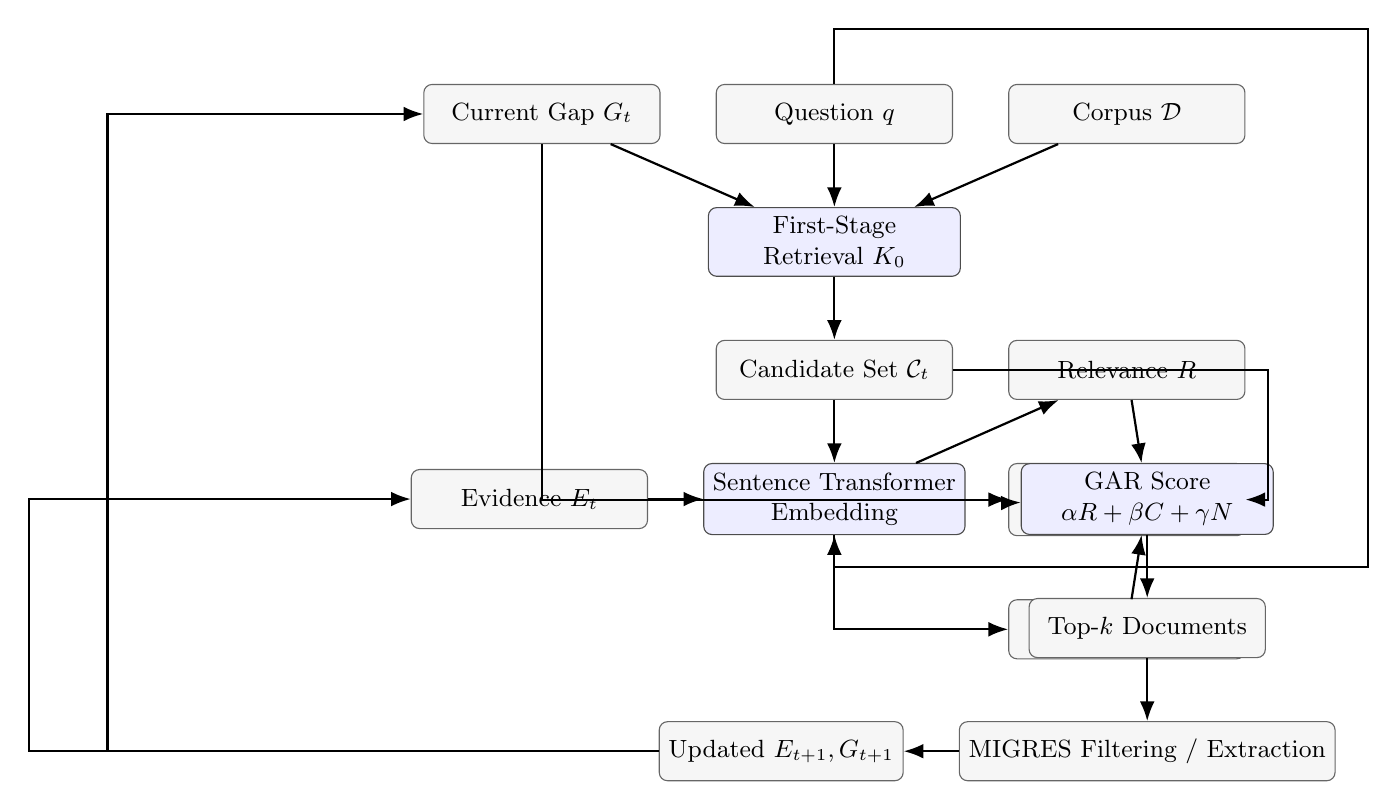
\begin{tikzpicture}[node distance=8mm and 7mm]

% Inputs
\node[block] (q) {Question $q$};
\node[block,left=of q] (g) {Current Gap $G_t$};
\node[block,right=of q] (d) {Corpus $\mathcal{D}$};

% First-stage retrieval
\node[important,below=of q] (fsr) {First-Stage\\Retrieval $K_0$};
\node[block,below=of fsr] (cand) {Candidate Set $\mathcal{C}_t$};

% Embedding, computed only over the candidate set (feeds Relevance and Novelty only)
\node[important,below=of cand] (emb) {Sentence Transformer\\Embedding};
\node[block,left=of emb] (e) {Evidence $E_t$};

% GAR components
\node[block,right=of cand] (r) {Relevance $R$};
\node[block,below=of r] (c) {Coverage $C$\\(token overlap)};
\node[block,below=of c] (n) {Novelty $N$};

% Final score
\node[important,right=of emb] (score)
    {GAR Score\\$\alpha R+\beta C+\gamma N$};

% Output and MIGRES
\node[block,below=of score] (top) {Top-$k$ Documents};
\node[block,below=of top] (mig) {MIGRES Filtering / Extraction};
\node[block,left=of mig] (next) {Updated $E_{t+1},G_{t+1}$};

% Inputs -> first-stage retrieval
\draw[arrow] (q) -- (fsr);
\draw[arrow] (g) -- (fsr);
\draw[arrow] (d) -- (fsr);

% First-stage retrieval -> candidate set
\draw[arrow] (fsr) -- (cand);

% Candidate set -> embedding (only Ct is embedded, not all of \mathcal{D})
% Relevance and Novelty use embeddings; Coverage uses raw candidate/gap text directly.
\draw[arrow] (cand) -- (emb);
\draw[arrow] (e) -- (emb);
\draw[arrow] (cand.east) -- ++(4,0) |- (c.east);
\draw[arrow] (g.south) |- (c.west);

% Question -> embedding (q is embedded so that R(d,q)=s(d,q) can be computed)
\draw[arrow] (q.north) -- ++(0,7mm) -| ([xshift=12mm,yshift=-4mm]score.east |- emb.south) -| (emb.south);

% Embedding -> Relevance and Novelty only
\draw[arrow] (emb) -- (r);
\draw[arrow] (emb) |- (n);

% Components -> final score
\draw[arrow] (r) -- (score);
\draw[arrow] (c) -- (score);
\draw[arrow] (n) -- (score);

% Final ranking -> MIGRES
\draw[arrow] (score) -- (top);
\draw[arrow] (top) -- (mig);

% MIGRES updates the state
\draw[arrow] (mig) -- (next);

% Feedback loop for next iteration
\draw[arrow] (next.west) -- ++(-7,0) |- (g.west);
\draw[arrow] (next.west) -- ++(-8,0) |- (e.west);

\end{tikzpicture}
\end{center}

\captionof{figure}{Overall architecture of GAR within the MIGRES framework. MIGRES provides the current question, evidence, and information gap. The selected first-stage retriever (Section~2) retrieves over the corpus $\mathcal{D}$ to produce the candidate set $\mathcal{C}_t$. Relevance and Novelty are computed from Sentence Transformer embeddings of the candidates, the question $q$ (for Relevance), and the collected evidence $E_t$ (for Novelty); Coverage is computed directly from candidate and gap text via token overlap and does not require embeddings. The reranked documents are then returned to MIGRES for filtering, extraction, and state updating.}

\subsection{Step 1: Dataset Question}

A benchmark supplies the original question:

\[
q.
\]

The benchmark's gold answer and supporting evidence are not given to GAR during retrieval.

\subsection{Step 2: MIGRES Creates the Retrieval State}

MIGRES processes the question and maintains:

\[
E_t=\text{evidence already collected}
\]

and:

\[
G_t=\text{information still missing}.
\]

The gap can contain multiple requirements:

\[
G_t=\{g_1,\ldots,g_m\}.
\]

GAR does not independently invent $G_t$ in the main experiment. It receives the gap produced by MIGRES.

\subsection{Step 3: First-Stage Retrieval}

The selected first-stage retriever (Section~2) operates directly on the raw text of $\mathcal{D}$; for the sparse lexical candidates considered here (e.g.\ BM25), it requires no embeddings. For each query-like input $x$, it returns the $K_0$ highest-scoring documents:

\[
\mathrm{FSR}_{K_0}(x,\mathcal{D}).
\]

GAR's candidate set is built using both the original question and every gap requirement, so that first-stage retrieval is itself gap-aware:

\[
\boxed{
\mathcal{C}_t
=
\mathrm{FSR}_{K_0}(q,\mathcal{D})
\cup
\bigcup_{i=1}^{m}
\mathrm{FSR}_{K_0}(g_i,\mathcal{D})
}
\tag{9}
\]

Duplicates are removed. Because each of the $m+1$ retrieval calls can return up to $K_0$ documents, the resulting candidate pool satisfies $|\mathcal{C}_t|\le(m+1)K_0$ after deduplication, not $|\mathcal{C}_t|=K_0$; $K_0$ is the retrieval depth used for each individual query, while $k$ is the final number of documents returned after reranking.

Taking the union in Eq.~(9) yields a set in which a document can appear in more than one of the $m+1$ retrieved lists with different first-stage scores under $q$ or a given $g_i$. These individual FSR scores are retained alongside $\mathcal{C}_t$ for the baselines that need them (LambdaMART's first-stage-score feature, whose value is the fused score defined below, and the fused ordering used by AIR and RankGPT), but they are not used in GAR's own score. GAR itself does not need these first-stage scores, as it rescoring every $d\in\mathcal{C}_t$ from scratch using $R$, $C$, and $N$. However, the no-reranking control (the selected first-stage retriever with no reranker) does need a defined top-$k$ over $\mathcal{C}_t$: for that system, we fuse a document's score as the maximum first-stage score it received across the retrieval calls that returned it, i.e.\ $\max\big(\mathrm{FSR}(d,q),\max_i \mathrm{FSR}(d,g_i)\big)$, and rank $\mathcal{C}_t$ by this fused score.

This step is cheap relative to embedding the full corpus even when $\mathcal{D}$ contains millions of documents, and it avoids requiring GAR to build or query a dense index over the full corpus.

\subsection{Step 4: Convert Candidate Text to Embeddings}

GAR uses the fixed Sentence Transformer model:

\[
\phi(x).
\]

The question, each evidence item, and \emph{only the documents already in $\mathcal{C}_t$} are represented as vectors for the relevance and novelty terms; gap requirements are not embedded and are processed by the token-overlap Coverage term. Because $|\mathcal{C}_t|\le(m+1)K_0\ll|\mathcal{D}|$, GAR never needs to embed or index the full corpus --- embeddings are computed on demand for the small candidate set returned by the first-stage retriever.

\subsection{Step 5: Calculate Relevance}

For every candidate:

\[
R(d,q)
\]

measures:

\[
\text{question-document relevance}.
\]

\subsection{Step 6: Calculate Coverage}

GAR then asks:

\[
\text{``Does this document cover the information that is missing?''}
\]

This produces:

\[
C(d,G_t).
\]

\subsection{Step 7: Calculate Novelty}

GAR then asks:

\[
\text{``Is this document redundant with evidence already collected?''}
\]

This produces:

\[
N(d,E_t).
\]

\subsection{Step 8: Calculate the GAR Score}

For every candidate:

\[
S(d\mid q,E_t,G_t)
=
\alpha R+\beta C+\gamma N.
\]

The candidate with the highest score is preferred because it is simultaneously relevant, gap-covering, and non-redundant.

\subsection{Step 9: Return Top-$k$}

GAR returns:

\[
\boxed{
T_t=
\operatorname{TopK}_{d\in\mathcal C_t}
S(d\mid q,E_t,G_t)
}
\tag{10}
\]

where $k$ is fixed for the experiment. Because $\mathcal{C}_t$ contains the question retrieval $\mathrm{FSR}_{K_0}(q,\mathcal{D})$, $K_0\ge k$ is sufficient to guarantee $|\mathcal{C}_t|\ge k$ when each retrieval returns $K_0$ documents, but it is not necessary: with $K_0<k$, the union of the question and gap retrievals can still contain at least $k$ unique candidates. When fewer than $k$ unique candidates exist, GAR returns all $\min(k,|\mathcal{C}_t|)$ of them, ranked by $S$.

\subsection{Step 10: MIGRES Continues}

MIGRES receives the retrieved documents and performs its normal filtering and extraction.

It updates:

\[
E_{t+1}
\]

and, if more information is needed:

\[
G_{t+1}.
\]

GAR is then called again.

The complete loop is:

\[
\boxed{
(q,E_t,G_t,\mathcal{D})
\xrightarrow{\mathrm{FSR}}
\mathcal{C}_t
\xrightarrow{\mathrm{GAR}}
T_t
\xrightarrow{\mathrm{MIGRES}}
(E_{t+1},G_{t+1})
\xrightarrow{\mathrm{FSR}}
\mathcal{C}_{t+1}
\xrightarrow{\mathrm{GAR}}
T_{t+1}
}
\]

This is why GAR is evaluated inside MIGRES rather than as an isolated one-shot reranker.

\subsection{Retrieval vs.\ Reranking in This Design}

The two stages must not be confused:

\[
\boxed{
\text{First-stage retrieval}
\rightarrow
\text{Embedding}
\rightarrow
\text{GAR scoring}
\rightarrow
\text{Top-}k
}
\]

The first-stage retriever finds a manageable candidate set from the full corpus $\mathcal{D}$.

Embedding converts only that candidate set (plus the question $q$ and the evidence $E_t$) into vectors; gap requirements $G_t$ are not embedded and are handled by token-overlap Coverage.

GAR makes the final ranking decision over the candidate set.

This is precisely the reranking design proposed in this project: a first-stage retriever narrows the corpus down to $\mathcal{C}_t$, and GAR reranks that output using relevance, gap coverage, and evidence novelty. A version of GAR that performs its own first-stage candidate generation directly from $\mathcal{D}$ (for example, via an ANN index over GAR's own embeddings, without relying on a separate first-stage retriever) would instead be a complete end-to-end retrieval algorithm; that variant is not evaluated here and is left as a direction for future work.

% ============================================================
\subsection{Development, Validation, and Test Protocol}

\subsubsection{Is GAR Trained?}

No.

The proposed GAR algorithm has no trainable parameters. We do not train GAR on $D_{\mathrm{train}}$.

The embedding model is a fixed pretrained Sentence Transformer. It is not fine-tuned in the primary experiment.

Therefore the experiment has no GAR training stage.

\subsubsection{Training Data}

If a baseline uses an official pretrained checkpoint, we use that checkpoint rather than retraining it on the evaluation data.

The benchmark training split may be used for auxiliary development or baseline-specific training only if required by the official implementation. Any such use must be documented, must not use test annotations, and follows the protocol of Section~\ref{sec:baseline-protocol}.

For GAR itself:

\[
D_{\mathrm{train}}
\not\rightarrow
\text{GAR parameter learning}.
\]

\subsubsection{Validation Set $D_{\mathrm{val}}$}

We define:

\[
\boxed{D_{\mathrm{val}}=\text{the held-out development/validation split}.}
\]

Where an official development split exists, we use it; where the official test annotations are withheld, the development split is divided into a validation half and a test half as described in Section~7.10. The exact files and split names are recorded for each dataset.

GAR hyperparameters are selected using the \emph{complete MIGRES+FSR+GAR pipeline} on $D_{\mathrm{val}}$.

This is important because GAR cannot be meaningfully validated in isolation: $E_t$ and $G_t$ are produced by the MIGRES iterative process, and $\mathcal{C}_t$ is produced by $\mathrm{FSR}$.

The validation loop is:

\[
D_{\mathrm{val}}
\rightarrow
\text{MIGRES}
\rightarrow
(q,E_t,G_t)
\rightarrow
\text{FSR}
\rightarrow
\mathcal{C}_t
\rightarrow
\text{GAR}
\rightarrow
\text{MIGRES}
\rightarrow
\text{validation metric}.
\]

\subsubsection{Bayesian Optimization}

We use Bayesian optimization to select:

\[
\theta_{\mathrm{GAR}}
=
\{\alpha,\beta,\gamma,K_0\}.
\]

Bayesian optimization uses previous validation evaluations to decide which configuration to test next rather than exhaustively evaluating every possible combination \citep{snoek2012practical}.

The search space is:

\[
\alpha,\beta,\gamma\geq0,
\qquad
\alpha+\beta+\gamma=1,
\]

and a predefined discrete candidate set for $K_0$, for example:

\[
K_0\in\{50,100,200,500\}.
\]

The exact search space and random seed are recorded before the experiment.

The optimization objective must be selected before test evaluation. The primary objective should be a retrieval metric aligned with the main research question, such as Recall@$k$ on $D_{\mathrm{val}}$.

The procedure is:

\[
\boxed{
D_{\mathrm{val}}
\rightarrow
\text{MIGRES+FSR+GAR}
\rightarrow
\text{validation score}
\rightarrow
\text{Bayesian optimization}
\rightarrow
\theta^*_{\mathrm{GAR}}
}
\]

The selected configuration is then frozen.

\subsubsection{Test Set $D_{\mathrm{test}}$}

After validation:

\[
\boxed{
\theta^*_{\mathrm{GAR}}
\text{ is frozen.}
}
\]

We then evaluate:

\[
D_{\mathrm{test}}
\rightarrow
\text{MIGRES+FSR+GAR}(\theta^*_{\mathrm{GAR}})
\rightarrow
\text{final metrics}.
\]

No test result is used to change the hyperparameters.

The same $k$, dataset, corpus, MIGRES configuration, and stopping conditions are used for the comparison systems wherever possible.

Because $K_0$ is one of the parameters selected by Bayesian optimization on $D_{\mathrm{val}}$ for GAR specifically (Section~6.13.4), and the same frozen $K_0$ then fixes the candidate pool $\mathcal{C}_t$ passed to every baseline reranker, the candidate-pool depth is not independently tuned for each baseline. This is a limitation of the comparison: it should be read as GAR vs.\ baselines under a candidate-pool depth chosen to favor GAR's own validation performance, not under a depth optimized separately for each system. A stricter design would either fix $K_0$ in advance independently of any reranker's performance, or tune each baseline's own hyperparameters (including its effective candidate depth, where applicable) on $D_{\mathrm{val}}$ under the same protocol used for GAR.

\subsubsection{Complete Experimental Flow}

\begin{enumerate}[leftmargin=1.5em]
\item Prepare the official dataset splits and searchable corpus.
\item Run the first-stage-retriever comparison (Section~2) on $D_{\mathrm{val}}$ and select $\mathrm{FSR}$ as the best-performing candidate; freeze $\mathrm{FSR}$ for every step below.
\item Reproduce MIGRES+FSR as the no-reranking control.
\item Verify the MIGRES retrieval interface and confirm how $E_t$ and $G_t$ are exposed.
\item Implement on-demand embedding of $\mathrm{FSR}$'s candidate set $\mathcal{C}_t$ using the fixed Sentence Transformer.
\item Implement and unit-test the GAR equations.
\item Run Bayesian optimization on $D_{\mathrm{val}}$ through the complete MIGRES+FSR+GAR pipeline.
\item Freeze $\alpha,\beta,\gamma,K_0$.
\item Run the held-out $D_{\mathrm{test}}$ with the frozen configuration.
\item Run MonoBERT, MonoT5, DuoBERT, ColBERTv2, LambdaMART, RankT5, MMR, AIR, Dartboard/RIG, and RankGPT as rerankers on the identical $\mathrm{FSR}$ candidate set, using their established implementations.
\item Evaluate retrieval quality, downstream answer quality, efficiency, and cost.
\item Run GAR ablations using the same frozen evaluation protocol.
\end{enumerate}

% ============================================================
\section{Datasets}

\subsection{Dataset Selection}

The project uses the six datasets reported in the MIGRES evaluation:

\[
\boxed{
\text{WikiHop},\;
\text{HotpotQA},\;
\text{MuSiQue},\;
\text{Natural Questions},\;
\text{TriviaQA},\;
\text{StrategyQA}
}
\]

These datasets provide questions and task-specific answer/evidence annotations suitable for evaluating retrieval and downstream question answering.

\subsection{WikiHop}

\textbf{Paper:} \citet{welbl-etal-2018-constructing}.

WikiHop is a multi-document, multi-hop reading-comprehension benchmark designed so that the answer requires combining information across documents. The dataset is useful for GAR because it tests whether retrieval can assemble complementary evidence rather than repeatedly retrieving one topic.

Typical fields include a question, candidate documents, an answer, and supporting information.

Paper:
\url{https://aclanthology.org/Q18-1021/}

\subsection{HotpotQA}

\textbf{Paper:} \citet{yang-etal-2018-hotpotqa}.

HotpotQA contains about 113K Wikipedia-based question-answer pairs and provides sentence-level supporting facts. It includes multi-hop and comparison questions \citep{yang-etal-2018-hotpotqa}.

For first-stage development, we use the FullWiki setting because it requires retrieval from a larger Wikipedia corpus. The official repository provides train, development, and FullWiki resources and explicitly allows researchers to replace its retrieval component with their own IR system.

Paper:
\url{https://aclanthology.org/D18-1259/}

Official resources:
\url{https://hotpotqa.github.io/}

The repository documentation describes the FullWiki development and test files and the use of custom IR systems.

\subsection{MuSiQue}

\textbf{Paper:} \citet{trivedi-etal-2022-musique}.

MuSiQue was designed to reduce shortcut solutions in multi-hop QA. MuSiQue-Ans contains about 25K questions requiring 2--4 hops \citep{trivedi-etal-2022-musique}.

Typical information includes a question, answer, reasoning structure, and supporting evidence.

Paper:
\url{https://aclanthology.org/2022.tacl-1.31/}

Official repository:
\url{https://github.com/StonyBrookNLP/musique}

\subsection{Natural Questions}

\textbf{Paper:} \citet{kwiatkowski-etal-2019-natural}.

Natural Questions consists of real anonymized queries issued to Google Search and Wikipedia-based annotations. The public release contains about 307K training examples, 7,830 development examples, and 7,842 sequestered test examples \citep{kwiatkowski-etal-2019-natural}. The exact training count is reported as 307,373 in the paper and in the data-statistics section of the official repository, while the repository's data-description paragraph gives 307,372; the count of the downloaded release is recorded in the experiment configuration.

Typical fields include a question, Wikipedia page information, long-answer annotations, short-answer annotations, and document-level information.

Paper:
\url{https://aclanthology.org/Q19-1026/}

Official research page:
\url{https://ai.google/research/NaturalQuestions}

\subsection{TriviaQA}

\textbf{Paper:} \citet{joshi-etal-2017-triviaqa}.

TriviaQA contains about 95K question-answer pairs and more than 650K question-answer-evidence triples. Questions were written by trivia enthusiasts and paired with independently gathered evidence documents \citep{joshi-etal-2017-triviaqa}.

Typical fields include a question, answer, aliases, and evidence documents.

Paper:
\url{https://aclanthology.org/P17-1147/}

Official resources:
\url{https://nlp.cs.washington.edu/triviaqa/}

\subsection{StrategyQA}

\textbf{Paper:} \citet{geva-etal-2021-strategyqa}.

StrategyQA contains 2,780 questions with implicit reasoning strategies. Each example includes a question, a reasoning decomposition, and Wikipedia evidence paragraphs \citep{geva-etal-2021-strategyqa}.

This makes it useful for testing whether gap-aware reranking helps when the required reasoning steps are not directly stated in the question.

Paper:
\url{https://aclanthology.org/2021.tacl-1.21/}

Official resources:
\url{https://allenai.org/data/strategyqa}

\subsection{Dataset Summary}

\begin{center}
\small
\begin{tabular}{p{2.7cm}p{2.5cm}p{7.3cm}}
\toprule
\textbf{Dataset} & \textbf{Scale} & \textbf{Useful properties for GAR}\\
\midrule
WikiHop & $\sim$51K & Multi-document, multi-hop reasoning.\\
HotpotQA & $\sim$113K & Multi-hop QA with sentence-level supporting facts; FullWiki retrieval.\\
MuSiQue & $\sim$25K & 2--4 hop compositional reasoning.\\
Natural Questions & $\sim$307K train; 7,830 dev; 7,842 test (withheld) & Real search questions with Wikipedia annotations.\\
TriviaQA & $\sim$95K QA pairs; $>$650K evidence triples & Heterogeneous evidence and lexical variation.\\
StrategyQA & 2,780 & Implicit reasoning with evidence paragraphs.\\
\bottomrule
\end{tabular}
\end{center}

Exact counts used in experiments must be taken from the downloaded release and recorded in the experiment configuration. Dataset counts can differ by release or preprocessing.

\subsection{What a Dataset Example Looks Like}

The common conceptual structure is:

\[
\boxed{
\text{Question}
+
\text{Corpus/Evidence}
+
\text{Answer}
+
\text{Ground-Truth Evidence/Annotations}
}
\]

For example, a HotpotQA-style example contains a natural-language question, an answer, supporting facts, and Wikipedia context. During reranking, GAR receives the question, MIGRES's evidence and gap state, and the candidate set already retrieved by $\mathrm{FSR}$ from the searchable corpus. The gold answer and gold supporting evidence are reserved for evaluation.

The ground-truth evidence must never be used to construct $G_t$, $E_t$, or the $\mathrm{FSR}$ candidate pool during test-time retrieval.

\subsection{Dataset Split Policy}

For each dataset:

\[
D_{\mathrm{train}},\quad
D_{\mathrm{val}},\quad
D_{\mathrm{test}}
\]

are treated separately where official splits are available.

For GAR:

\[
D_{\mathrm{val}}
\]

is used for hyperparameter optimization, while:

\[
D_{\mathrm{test}}
\]

is used only for the final evaluation.

\textbf{Labelled test data.} The retrieval metrics of this project (Recall, Precision, MRR, nDCG, GapEvidenceCoverage, and $\mathrm{CandRecall}$) need ground-truth evidence annotations, and these are withheld for some official test sets. For Natural Questions the 7,842 test examples are withheld and can only be scored through the official competition site, and the HotpotQA FullWiki test set is released without answers or supporting facts. This is checked for every dataset and recorded in the experiment configuration. For any dataset whose official test annotations are unavailable, $D_{\mathrm{val}}$ and $D_{\mathrm{test}}$ are two disjoint, question-level halves of the labelled official development split, divided once with a recorded seed before any experiment is run. Neither half is used to train or tune any system except $D_{\mathrm{val}}$ for the selections described in Section~\ref{sec:e1} and Section~6.13, and the official training split may be used only for baseline-specific training under Section~\ref{sec:baseline-protocol}. All retrieval metrics and all confirmatory tests are computed on this labelled $D_{\mathrm{test}}$.

Official hidden-test evaluation is optional. If it is performed, it yields only the end-to-end answer metrics returned by the official evaluation procedure (no retrieval metrics), is run once per system with the frozen configuration, and is reported separately rather than pooled with the labelled $D_{\mathrm{test}}$ analyses.

% ============================================================
\section{Experimental Design and Analysis}
\label{sec:expdesign}

This section is the complete experimental protocol of the project. It fixes, before any $D_{\mathrm{test}}$ result is inspected, which systems are compared, which research questions and hypotheses are tested, which metrics are computed, how the ablations are run, and how the statistics are carried out. It does not modify the GAR formulation of Sections~5 and~6 (Eqs.~(1)--(10)), the MIGRES setup of Section~1, or the datasets of Section~7, and it reports no results: every statement below about performance is a question or a hypothesis, not a finding.

Throughout, $\mathrm{FSR}$ is the first-stage retriever selected in Experiment~E1, $\mathcal{C}_t$ is the candidate set of Eq.~(9), $K_0$ is the per-query retrieval depth, $k$ is the final retrieval depth returned to MIGRES, and $D_{\mathrm{val}}$, $D_{\mathrm{test}}$ are the validation and test splits of the six datasets of Section~7. All experiments are run separately on each of the six datasets; ``across datasets'' always means the macro-average over the six.

% ------------------------------------------------------------
\subsection{Experimental Objectives}
\label{sec:obj}

The experimental study has four purposes:

\begin{enumerate}[leftmargin=1.5em]
\item to compare first-stage information retrieval algorithms;
\item to compare GAR with established reranking algorithms on the same candidate set;
\item to determine which GAR components contribute to performance, through ablation;
\item to measure downstream question-answering quality, computational cost, and robustness (across datasets and across candidate-pool depths).
\end{enumerate}

These purposes correspond to two different kinds of experiment, which are never mixed:

\begin{center}
\small
\begin{tabularx}{\textwidth}{>{\raggedright\arraybackslash}p{2.5cm}>{\raggedright\arraybackslash}X>{\raggedright\arraybackslash}X}
\toprule
 & \textbf{First-stage retrieval (E1)} & \textbf{Reranking (E2--E5)}\\
\midrule
Input & The question $q$ alone; the full corpus $\mathcal{D}$. & The fixed candidate set $\mathcal{C}_t$ built by the frozen $\mathrm{FSR}$ (Eq.~(9)), together with $q$, $E_t$, $G_t$.\\
Output & A ranked list over $\mathcal{D}$ of depth $K_0$. & A reordering of $\mathcal{C}_t$; no document outside $\mathcal{C}_t$ can be returned.\\
Systems & BM25, DPR, Contriever, ColBERTv2, SPLADE. & $\mathrm{FSR}$ (no reranking), ten rerankers, GAR.\\
GAR present? & No. & Yes.\\
Purpose & Select $\mathrm{FSR}$ on $D_{\mathrm{val}}$. & Test GAR, its components, its sensitivity to $K_0$, and its cost.\\
\bottomrule
\end{tabularx}
\end{center}

ColBERTv2 appears in both roles with different configurations: in E1 it searches the corpus $\mathcal{D}$ as a first-stage retriever; in E2 it only rescores the documents already in $\mathcal{C}_t$, as described in Section~3.

% ------------------------------------------------------------
\subsection{Experiment E1: First-Stage Information Retrieval Comparison}
\label{sec:e1}

\textbf{Systems.}
\[
\text{BM25},\quad \text{DPR},\quad \text{Contriever},\quad \text{ColBERTv2},\quad \text{SPLADE}.
\]
These methods are compared \emph{only} as candidate-generation (first-stage) retrieval systems, using their published or official implementations and checkpoints where possible (Section~2).

\textbf{Protocol.} All five systems are evaluated under the same conditions:
\begin{itemize}[leftmargin=1.5em]
\item the same dataset split ($D_{\mathrm{val}}$ of each dataset);
\item the same questions;
\item the same searchable corpus $\mathcal{D}$;
\item the same per-query retrieval depth: every system returns its top $500$ documents for each query, the largest value of the grid of Section~\ref{sec:e4}, so that every shallower depth $\{50,100,200\}$ is obtained by truncating the same ranked list. The depth used for \emph{selection} is fixed in advance as $K_0^{\mathrm{sel}}=100$ (the grid value nearest the middle of the range); it is not tuned on any result, and it is distinct from the $K_0$ later tuned for GAR (Section~5.8);
\item GAR is not used in this experiment, and no MIGRES reranking is applied;
\item gold answers and gold supporting evidence are never used during retrieval; they are used only to score the returned lists.
\end{itemize}
\textbf{Candidate construction and reference trajectory.} E1 follows the same candidate-construction procedure as the main experiment. For every $D_{\mathrm{val}}$ question, MIGRES with its original retriever (BM25) and no reranking is run once, and $(q,E_t,G_t)$ is stored for every iteration $t$; no LLM call is repeated per candidate retriever. Each candidate retriever $\rho$ then builds
\[
\mathcal{C}_t^{\rho}=\rho_{K_0}(q,\mathcal{D})\cup\bigcup_{i=1}^{m}\rho_{K_0}(g_i,\mathcal{D})
\]
(Eq.~(9)) from these stored queries, with duplicates removed and no further truncation. Because the stored gaps come from a trajectory produced with BM25 retrieval, this design may favour lexical retrievers slightly; the reference trajectory is recorded so this can be inspected. E1 also reports the question-only ranking $\rho_{K_0}(q,\mathcal{D})$ and the mean and maximum pool size $|\mathcal{C}_t^{\rho}|$ as diagnostics; only the union measurement is used for selection.

\textbf{Retrieval-quality metrics.} The selection metric is $\mathrm{CandRecall}@K_0^{\mathrm{sel}}$. For reference, the question-only ranking of every system is also scored with Recall@$k$; MRR@10; nDCG@10; and Precision@$k$, wherever the dataset annotations support binary relevance. Recall@$k$ is reported at the final depth $k$ and at each depth in $\{50,100,200,500\}$. Definitions are given in Section~\ref{sec:metric-defs}.

\textbf{Cost measurements.} For each system we also report retrieval latency per query, indexing time, index memory, and the number of retrieved candidates ($K_0^{\mathrm{E1}}$), on the same recorded hardware.

\textbf{Selection rule.} The primary purpose of E1 is to select $\mathrm{FSR}$ on $D_{\mathrm{val}}$. The system with the highest macro-averaged (across the six datasets) candidate-pool recall $\mathrm{CandRecall}@K_0^{\mathrm{sel}}$ on $D_{\mathrm{val}}$ (Section~\ref{sec:metric-defs}) is selected; it is chosen because candidate generation must not lose the evidence that later stages need, and it measures exactly the candidate set $\mathcal{C}_t$ that every reranker will receive. Because a larger pool trivially raises recall, the mean pool size is reported next to it. If two systems tie at the reported precision, the tie is broken by smaller mean pool size, and then by lower latency. The selected system is frozen as $\mathrm{FSR}$ and used unchanged in E2--E5.

\textbf{What E1 does and does not show.} E1 does \emph{not} test GAR and is not evidence that GAR is effective. It only determines the fixed retrieval substrate on which the reranking study is run.

% ------------------------------------------------------------
\subsection{Experiment E2: Main Reranking Comparison}
\label{sec:e2}

\textbf{Candidate set.} After $\mathrm{FSR}$ is selected, the candidate set $\mathcal{C}_t$ is constructed once per question and iteration by Eq.~(9), with the validation-selected $K_0$ (Section~6.13.5). \textbf{Every reranker receives the identical candidate set $\mathcal{C}_t$ for the same question and iteration.} The only intended experimental variable is the reranking method.

\textbf{Systems.}
\[
\begin{aligned}
&\text{FSR (no reranking)},\; \text{MonoBERT},\; \text{MonoT5},\; \text{DuoBERT},\; \text{ColBERTv2},\; \text{LambdaMART},\\
&\text{RankT5},\; \text{MMR},\; \text{AIR},\; \text{Dartboard/RIG},\; \text{RankGPT},\; \text{GAR}.
\end{aligned}
\]
The no-reranking control ranks $\mathcal{C}_t$ by the fused score $\max\big(\mathrm{FSR}(d,q),\max_i \mathrm{FSR}(d,g_i)\big)$ (Section~6.4). Each reranker is used in the form described in Section~3, including the adaptations of AIR and RankGPT to the common candidate set. Every reranker outputs a complete ordering of $\mathcal{C}_t$ (the greedy methods MMR, AIR, and Dartboard/RIG continue their selection until $\mathcal{C}_t$ is exhausted).

\textbf{Matched-state retrieval evaluation.} Because $(E_t,G_t)$ depend on the documents returned in earlier iterations, live runs of different rerankers diverge after the first iteration and would then no longer reorder the same $\mathcal{C}_t$. To enforce identical inputs, the \emph{retrieval} metrics of E2--E4 are computed in matched-state mode: the MIGRES$+\mathrm{FSR}$ (no reranking) run is recorded once per question, storing $(q,E_t,G_t,\mathcal{C}_t)$ for every iteration $t$; each system then reorders exactly this stored $\mathcal{C}_t$, and the metrics are computed on its ordering. The \emph{downstream} metrics are computed in live mode: each system is run end to end inside MIGRES with only the reranking method replaced. Retrieval metrics are also logged in the live runs as a secondary analysis. Each retrieval call (question $i$, iteration $t$) yields one ranked list and one score per metric; the score of question $i$ is the mean over its iterations, and the question is the unit of analysis in all statistics (Section~\ref{sec:stats}).

\textbf{Retrieval metrics over iterations.} The primary retrieval metrics are \emph{per-iteration}: at each iteration $t$ they are computed on the system's ordering of $\mathcal{C}_t$ against the full set of ground-truth relevant evidence, and evidence found at earlier iterations is not removed from that set. The per-iteration scores are then averaged over the iterations of the question. In matched-state mode the number of iterations is the one recorded in the no-reranking run, for every system. As a secondary \emph{cumulative} measure, we also report Recall over the union of the top-$k$ lists returned across all iterations, in which a document returned in several iterations is counted once. In the live runs the iterations actually performed by each system are used, so live retrieval metrics are not paired at the iteration level.

\textbf{Primary ranking metrics.} All twelve systems are evaluated with the same metrics,
\[
\boxed{\text{Recall@}k,\;\; \text{MRR@10},\;\; \text{nDCG@10},\;\; \text{Precision@}k}
\]
with the same $k$ for all systems. Recall@$k$ and Precision@$k$ use the final depth $k$; MRR@10 and nDCG@10 use cutoff $10$ on the system's full ordering of $\mathcal{C}_t$ and are therefore defined for every $k$.

\textbf{Complementary metrics.} We additionally report GapEvidenceCoverage@$k$ as a GAR-specific complementary metric where the dataset annotations permit the mapping from annotations to evidence requirements; downstream answer EM; downstream answer F1; classification accuracy for datasets where accuracy is the official task metric; and supporting-fact/evidence quality where the official annotations permit it (for example the sentence-level supporting facts of HotpotQA).

\textbf{Purpose of each metric.}
\begin{itemize}[leftmargin=1.5em]
\item \emph{Recall@$k$}: whether the required evidence enters the returned set;
\item \emph{MRR@10}: whether useful evidence appears very early in the ranking;
\item \emph{nDCG@10}: ranking quality when relevance has a graded structure (with binary annotations it is a position-discounted binary measure);
\item \emph{Precision@$k$}: how concentrated relevant evidence is in the returned set;
\item \emph{GapEvidenceCoverage@$k$}: whether the currently missing requirements are actually covered;
\item \emph{EM / F1 / accuracy}: whether improved retrieval translates into improved final answers.
\end{itemize}

The shared metrics are not replaced by different metrics for individual rerankers merely because their original publications used different benchmark setups (Section~\ref{sec:metrics-lit}).

% ------------------------------------------------------------
\subsection{Experiment E3: GAR Ablation Study}
\label{sec:e3}

The full GAR score is Eq.~(7),
\[
\boxed{S=\alpha R+\beta C+\gamma N.}
\]
Four variants are evaluated against it.

Without relevance:
\[
\boxed{S_{-R}=\beta C+\gamma N}
\]
Without coverage:
\[
\boxed{S_{-C}=\alpha R+\gamma N}
\]
Without novelty:
\[
\boxed{S_{-N}=\alpha R+\beta C}
\]
Relevance-only diagnostic:
\[
\boxed{GAR_{R\text{-only}}=R.}
\]

\textbf{Fixed conditions.} All evaluation conditions are held fixed: the same $\mathrm{FSR}$, candidate sets $\mathcal{C}_t$, questions, corpus, MIGRES configuration, and final $k$. Every variant uses the same frozen $\alpha,\beta,\gamma,K_0,k$ from the full GAR configuration (Section~6.13.5). The remaining weights are \emph{not} renormalized after a component is removed: dividing by the sum of the retained weights would multiply every candidate's score by the same positive constant and therefore would not change the ranking. An ablation is degenerate only if the retained weights sum to zero (for example $\beta+\gamma=0$ for $S_{-R}$), in which case every candidate receives the same score of zero. $GAR_{R\text{-only}}$ ranks by $R(d,q)$ alone, which is equivalent to $\alpha=1$, $\beta=\gamma=0$ (any positive $\alpha$ gives the same ranking).

\textbf{Metrics.} The ablations are evaluated with the same retrieval metrics (matched-state mode) and downstream metrics (live mode) as E2.

\textbf{Interpretation.}
\begin{itemize}[leftmargin=1.5em]
\item $S_{-R}$ measures the contribution of question relevance;
\item $S_{-C}$ measures the contribution of gap coverage;
\item $S_{-N}$ measures the contribution of evidence novelty;
\item $GAR_{R\text{-only}}$ provides a query-relevance baseline inside the GAR formulation. Together with $S_{-N}$ (relevance plus coverage), it helps separate the benefit of adding gap coverage from the benefit of the full relevance--coverage--novelty combination.
\end{itemize}

% ------------------------------------------------------------
\subsection{Experiment E4: Candidate-Pool Sensitivity}
\label{sec:e4}

E4 evaluates the effect of the first-stage candidate depth,
\[
K_0\in\{50,100,200,500\},
\]
on $D_{\mathrm{val}}$ only. For each $K_0$, the candidate set $\mathcal{C}_t$ is rebuilt by Eq.~(9) and GAR is run with $\alpha,\beta,\gamma$ held at their validation-selected values, which isolates the effect of candidate depth. We report Recall@$k$, MRR@10, nDCG@10, GapEvidenceCoverage@$k$, reranking latency, and the number of candidates scored $|\mathcal{C}_t|\le(m+1)K_0$.

The value $K_0$ used in the final test experiments is the one selected by the Bayesian-optimization procedure of Section~6.13.4; E4 does not re-select it. E4 is a \emph{sensitivity analysis}, not a separate final comparison: no $D_{\mathrm{test}}$ data are used, and no hypothesis of E2 or E3 is tested with it.

% ------------------------------------------------------------
\subsection{Experiment E5: Efficiency and Cost Analysis}
\label{sec:e5}

E5 compares GAR with the reranking baselines on $D_{\mathrm{test}}$, under the frozen configuration and recorded hardware, on:
\begin{itemize}[leftmargin=1.5em]
\item first-stage retrieval latency;
\item reranking latency;
\item end-to-end retrieval latency (first stage plus reranking);
\item number of documents scored;
\item number of model forward passes;
\item number of LLM calls;
\item input and output tokens;
\item API cost where applicable;
\item index-construction time (of $\mathrm{FSR}$, and separately any reranker-specific preprocessing, training, or index);
\item memory usage where applicable.
\end{itemize}

\textbf{Separation of costs.} Three quantities are always reported separately and never summed silently:
\begin{enumerate}[leftmargin=1.5em]
\item \emph{local retrieval/reranking computation} (the $\mathrm{FSR}$ and the reranker, on local hardware);
\item \emph{LLM cost of the reranker} (nonzero only for LLM-based rerankers, e.g.\ RankGPT);
\item \emph{LLM cost of the surrounding MIGRES system} (gap identification, extraction, and solving).
\end{enumerate}
The MIGRES cost is reported for every system, because a reranker can change the number of iterations and therefore the number of MIGRES LLM calls. Token counts, calls, and prices follow the cost model
\[
\boxed{
Cost(q)
=
\sum_{\ell\in\mathcal{L}(q)}
\Big(
T_{\mathrm{in}}(\ell)p_{\mathrm{in}}(\ell)
+
T_{\mathrm{out}}(\ell)p_{\mathrm{out}}(\ell)
\Big),
\qquad
\overline{Cost}=\frac{1}{N}\sum_{i=1}^{N}Cost(q_i),
}
\]
where $\mathcal{L}(q)$ is the set of LLM calls made while answering question $q$, $T_{\mathrm{in}}(\ell),T_{\mathrm{out}}(\ell)$ are the input/output tokens of call $\ell$, and $p_{\mathrm{in}}(\ell),p_{\mathrm{out}}(\ell)$ are the per-token prices of whichever model served that call. Because calls need not share a model or a price, the cost is summed per call; it reduces to $T_{\mathrm{in}}p_{\mathrm{in}}+T_{\mathrm{out}}p_{\mathrm{out}}$ only when $|\mathcal{L}(q)|=1$.

\textbf{Counting rules.} Pointwise rerankers (MonoBERT, MonoT5, RankT5) require one forward pass per candidate; DuoBERT requires $|\mathcal{C}_t|(|\mathcal{C}_t|-1)$ model calls (Section~3). GAR embeds the question, the evidence items in $E_t$, and only the documents in $\mathcal{C}_t$ with the fixed Sentence Transformer; these are local encoder passes, and gap coverage and novelty are computed locally by token overlap and cosine similarity. \textbf{GAR itself does not require one LLM call per candidate}; in the proposed implementation its scorer makes no LLM call. GAR also has no training stage and no corpus-wide embedding index (Sections~5.2 and~6.13.1). All counts are measured by instrumentation of the running systems rather than assumed.

E5 is descriptive: costs are reported as per-question means with 95\% bootstrap confidence intervals, and no significance test is part of the confirmatory protocol.

% ------------------------------------------------------------
\subsection{Research Questions}
\label{sec:rq}

\textbf{RQ1.} How do BM25, DPR, Contriever, ColBERTv2, and SPLADE compare as first-stage retrievers on the target datasets? \hfill (E1)

\textbf{RQ2.} Does GAR improve retrieval quality over the same $\mathrm{FSR}$ candidate set without reranking? \hfill (E2)

\textbf{RQ3.} How does GAR compare with established reranking methods when all methods rerank the identical candidate set? \hfill (E2)

\textbf{RQ4.} Does improved retrieval under GAR translate into improved downstream MIGRES answer quality? \hfill (E2)

\textbf{RQ5.} Which GAR components---relevance, gap coverage, or novelty---contribute to its performance? \hfill (E3)

\textbf{RQ6.} How does GAR performance change as the first-stage candidate-pool depth $K_0$ changes? \hfill (E4)

\textbf{RQ7.} What computational and API-cost trade-offs does GAR introduce relative to the baseline rerankers? \hfill (E5)

\textbf{RQ8.} Does the behavior of GAR remain consistent across the six datasets? \hfill (E2, E3)

% ------------------------------------------------------------
\subsection{Hypotheses}
\label{sec:hyp}

Each hypothesis corresponds to one experiment. None predicts a numerical improvement, and none asserts that GAR outperforms every baseline; where the outcome is uncertain, the hypothesis is an empirical question resolved by the statistics of Section~\ref{sec:stats}.

\textbf{H1 --- First-stage retrieval (E1).} The five first-stage retrieval algorithms exhibit different retrieval-quality performance on the validation datasets.

\textbf{H2 --- GAR vs.\ no reranking (E2).} GAR improves the primary retrieval metric (Recall@$k$) over the fixed $\mathrm{FSR}$ without reranking. This is the single confirmatory hypothesis.

\textbf{H3 --- GAR vs.\ reranking baselines (E2).} GAR achieves different ranking performance from established reranking methods when evaluated on the same candidate set. The comparator for the directional comparison, the best validation-selected baseline $B^\star$ (Section~\ref{sec:stats}), and the direction of the contrast ($\Delta=\text{GAR}-B^\star$) are fixed before $D_{\mathrm{test}}$ is evaluated.

\textbf{H4 --- Downstream QA (E2).} Improvements in retrieval quality under GAR are associated with improvements in downstream MIGRES answer quality.

\textbf{H5 --- Coverage contribution (E3).} Removing the coverage component decreases gap-evidence coverage and/or overall retrieval quality.

\textbf{H6 --- Novelty contribution (E3).} Removing the novelty component increases redundancy and decreases retrieval quality or evidence coverage.

\textbf{H7 --- Relevance contribution (E3).} Removing the relevance component decreases ranking quality with respect to the original question.

\textbf{H8 --- Candidate-pool sensitivity (E4).} GAR performance changes as $K_0$ changes, with larger candidate pools potentially increasing computational cost.

\textbf{Operationalization.} H1: pairwise differences among the five retrievers on $D_{\mathrm{val}}$, on $\mathrm{CandRecall}@K_0^{\mathrm{sel}}$. H2: GAR vs.\ $\mathrm{FSR}$ on Recall@$k$. H3: GAR vs.\ each reranker on Recall@$k$. H4: GAR vs.\ $\mathrm{FSR}$ on the official answer metric, and the association between per-question retrieval change and per-question answer-metric change (Section~\ref{sec:stats}). H5: Full GAR vs.\ $S_{-C}$ on GapEvidenceCoverage@$k$ and on Recall@$k$; supported if a decrease is established on at least one of them. H6: Full GAR vs.\ $S_{-N}$; supported if $S_{-N}$ has higher Redundancy@$k$ (Section~\ref{sec:metric-defs}) \emph{and} lower Recall@$k$ or lower GapEvidenceCoverage@$k$. H7: Full GAR vs.\ $S_{-R}$ on MRR@10 and nDCG@10, together with Recall@$k$. H8: GAR on $D_{\mathrm{val}}$ at each $K_0$ against the selected $K_0$, together with the measured reranking cost.

% ------------------------------------------------------------
\subsection{Primary and Secondary Metrics}
\label{sec:metrics}

\subsubsection{Metric hierarchy}

\begin{center}
\small
\begin{tabularx}{\textwidth}{>{\raggedright\arraybackslash}p{3.0cm}>{\raggedright\arraybackslash}X>{\raggedright\arraybackslash}X}
\toprule
\textbf{Evaluation level} & \textbf{Primary metrics} & \textbf{Secondary metrics}\\
\midrule
First-stage retrieval & $\mathrm{CandRecall}@K_0^{\mathrm{sel}}$ (Eq.~(9) pool) & Question-only Recall@$k$, MRR@10, nDCG@10; mean pool size; latency\\
Reranking & Recall@$k$, MRR@10, nDCG@10 & Precision@$k$, GapEvidenceCoverage@$k$\\
Downstream QA & Official dataset answer metric & EM, F1, accuracy, supporting-fact quality where applicable\\
Efficiency & End-to-end latency & Memory, indexing time, documents scored, tokens, API cost\\
\bottomrule
\end{tabularx}
\end{center}

The same ranking metrics are applied to \emph{all} rerankers, regardless of which metrics were used in their original publications. Of the three primary ranking metrics, Recall@$k$ is the single pre-registered confirmatory metric (Section~\ref{sec:stats}); it is also the objective used to select GAR's hyperparameters on $D_{\mathrm{val}}$ (Section~6.13.4). MRR@10 and nDCG@10 are reported with the same intervals but as secondary contrasts.

\subsubsection{Motivation from the original publications}
\label{sec:metrics-lit}

Before fixing the suite, we checked which metrics the primary publications of the compared methods actually report. Table~\ref{tab:metrics-lit} records what was verified; it is used only to justify the common suite, not to reproduce each paper's setup.

\begin{table}[H]
\centering
\small
\begin{tabularx}{\textwidth}{>{\raggedright\arraybackslash}p{2.6cm}>{\raggedright\arraybackslash}X}
\toprule
\textbf{Method (source)} & \textbf{Ranking / QA metrics reported in the original publication}\\
\midrule
MonoBERT \citep{nogueira-cho-2019-passage,nogueira-etal-2019-multistage} & MRR@10 (MS MARCO passage); MAP (TREC-CAR).\\
MonoT5 \citep{nogueira-etal-2020-document} & MRR@10 (MS MARCO passage); MAP and nDCG@20 (zero-shot TREC Robust04).\\
DuoBERT \citep{nogueira-etal-2019-multistage} & MRR@10 (MS MARCO); MAP (TREC-CAR).\\
ColBERTv2 \citep{santhanam-etal-2022-colbertv2} & MRR@10 and Recall@$k$ (MS MARCO, in domain); nDCG@10 (BEIR); Success@5 (LoTTE).\\
LambdaMART \citep{burges-2010-lambdamart} & Algorithmic overview without a benchmark metric suite; the method is presented as optimizing rank measures such as NDCG.\\
RankT5 \citep{zhuang-etal-2023-rankt5} & MRR@10 and nDCG@5, nDCG@10 (MS MARCO and Natural Questions dev sets, reranking the top-1000 of a dual encoder).\\
MMR \citep{carbonell-goldstein-1998-mmr} & Two-page poster with preliminary retrieval and summarization results; no standardized ranking-metric suite.\\
AIR \citep{yadav-etal-2020-unsupervised} & Evidence selection: precision, recall, and F1 (MultiRC) and Recall@10 (QASC); downstream QA performance.\\
Dartboard \citep{pickett-etal-2024-rig} & nDCG for the retrieval component and end-to-end QA correctness (Retrieval-Augmented Generation Benchmark).\\
RankGPT \citep{sun-etal-2023-chatgpt} & nDCG@1, nDCG@5, nDCG@10 (TREC, BEIR, Mr.\,TyDi).\\
\bottomrule
\end{tabularx}
\caption{Metrics reported by the original publications of the compared methods, as verified from the primary publications for this study.}
\label{tab:metrics-lit}
\end{table}

The publications use different benchmarks, cutoffs, and metric sets, so reproducing every original metric would make the cross-method comparison incoherent. We therefore adopt a common ranking core that each family of methods already supports:
\begin{itemize}[leftmargin=1.5em]
\item \textbf{MRR@10} is the headline metric of the BERT- and T5-based rerankers (MonoBERT, DuoBERT, MonoT5, RankT5) and is also reported for ColBERTv2;
\item \textbf{nDCG@10} is reported by RankT5, ColBERTv2 (BEIR), and RankGPT (which also reports nDCG@1 and nDCG@5), and nDCG is the retrieval metric of Dartboard; it also accommodates graded relevance where annotations provide it;
\item \textbf{Recall@$k$} is reported by ColBERTv2 and AIR (Recall@10) and is the metric most directly aligned with GAR's purpose, retrieving evidence that is still missing;
\item \textbf{Precision@$k$} is a complementary measure, consistent with the precision-based evidence-selection evaluation of AIR;
\item \textbf{Downstream answer metrics} (EM, F1, accuracy, supporting-fact quality) follow the practice of AIR and Dartboard of assessing retrieval by its effect on question answering, and are needed because MIGRES is evaluated end to end.
\end{itemize}
MAP, nDCG@20, nDCG@1/5, and Success@$k$ appear in individual papers but are not part of the common suite; they can be computed offline from the saved rankings as supplementary analyses without changing any confirmatory result.

\subsubsection{Metric definitions}
\label{sec:metric-defs}

The unit of retrieval is the document unit used in the MIGRES corpus. Relevance judgments come from each dataset's official evidence annotations, as recorded in the experiment configuration (Section~7); they are binary unless the annotation is graded, and the ground truth is used only for scoring.

\paragraph{Recall@$k$.}
Recall@$k$ measures how much of the ground-truth relevant evidence appears in the first $k$ retrieved documents:
\[
\boxed{
Recall@k
=
\frac{
|\text{relevant evidence}\cap\text{top-}k|
}{
|\text{relevant evidence}|
}
}
\]
Benchmarks used here provide at least one relevant-evidence item per question, so this denominator is not expected to be zero in practice; if an instance with no annotated relevant evidence does occur, that instance is excluded from the Recall@$k$ average (for all systems alike) rather than reported as $0/0$.

\paragraph{Candidate-pool recall (E1 only).}
$\mathrm{CandRecall}@K_0$ is the fraction of ground-truth relevant evidence contained in the full candidate set $\mathcal{C}_t^{\rho}$ built by Eq.~(9) at per-query depth $K_0$ for a candidate retriever $\rho$ (Section~\ref{sec:e1}); it is computed per iteration and averaged over the iterations of a question, and the same exclusion rule for questions without annotated evidence applies. It is a property of an unordered set, so it is not a ranking metric.

\paragraph{Precision@$k$.}
\[
\boxed{
Precision@k
=
\frac{
|\text{relevant documents in top-}k|
}{
k
}
}
\]

\paragraph{MRR and MRR@10.} Mean Reciprocal Rank measures how early the first relevant result appears:
\[
\boxed{
MRR
=
\frac{1}{N}
\sum_{i=1}^{N}
\frac{1}{rank_i}
}
\]
where $rank_i$ is the rank of the first relevant result for question $i$. For MRR@10, $\frac{1}{rank_i}$ is set to $0$ whenever no relevant document appears in the first $10$ results, following standard practice.

\paragraph{nDCG@$k$.} For graded relevance:
\[
DCG@k
=
\sum_{i=1}^{k}
\frac{2^{rel_i}-1}{\log_2(i+1)},
\qquad
\boxed{
nDCG@k
=
\frac{DCG@k}{IDCG@k}
}
\]
where $IDCG@k$ is the ideal DCG at cutoff $k$; nDCG@10 is the case $k=10$. The cumulated-gain idea is due to \citet{jarvelin-kekalainen-2002}; the exponential-gain form $2^{rel_i}-1$ with a $\log_2(i+1)$ discount used here is the variant common in learning to rank \citep{burges-2005-ranknet}, and differs from the linear-gain, $\log_b$-discount definition of the original paper. If $IDCG@k=0$ (no relevant document exists for that question), we define $nDCG@k=0$ for that question rather than leaving the ratio undefined.

\paragraph{GapEvidenceCoverage@$k$.} Because GAR explicitly models an information gap, we additionally report an evidence-coverage measure where the dataset annotations permit it:
\[
\boxed{
GapEvidenceCoverage@k
=
\frac{
\text{ground-truth evidence requirements retrieved in top-}k
}{
\text{total ground-truth evidence requirements}
}
}
\]
The exact mapping from benchmark annotations to evidence requirements is defined separately for each dataset and recorded in the experiment configuration before $D_{\mathrm{test}}$ is evaluated; for a dataset where no such mapping is possible the metric is not reported. As with Recall@$k$, an instance with zero total ground-truth evidence requirements is excluded from the average rather than reported as $0/0$.

\paragraph{Redundancy@$k$ (diagnostic for H6 only).} H6 concerns redundancy, which none of the metrics above measures. For a returned set $T$ and evidence $E_t\neq\varnothing$ we define, with the token normalization $\tau(\cdot)$ of Eq.~(3),
\[
Redundancy@k
=
\frac{1}{|T|}\sum_{d\in T}\max_{e\in E_t}
\frac{|\tau(d)\cap\tau(e)|}{|\tau(d)\cup\tau(e)|},
\qquad T=\text{top-}k.
\]
It is a lexical overlap measure, deliberately different from the embedding-based novelty term of Eq.~(5) so that it does not favor GAR by construction. It is undefined when $E_t=\varnothing$ (first iteration), and such calls are excluded. It is used only for the ablation contrast of H6 and is not part of the ranking metric suite.

\subsubsection{Downstream QA metrics}
\label{sec:downstream}

The final MIGRES answer is evaluated with the metrics supported by each benchmark, using the official evaluation script whenever one is available: Exact Match (EM); token-level F1; answer accuracy for classification-style datasets; and evidence/supporting-fact quality where annotations permit. For a benchmark with a normalized answer set $A_i$,
\[
EM_i=\mathbf{1}[\hat a_i\in A_i],
\qquad
EM=\frac{1}{N}\sum_{i=1}^{N}EM_i,
\qquad
F1=\frac{2PR}{P+R},
\]
where $P$ and $R$ are the precision and recall over normalized answer tokens. $F1$ is undefined when $P+R=0$; we adopt the convention of the benchmark's official evaluation script for this case (typically $F1=1$ if both predicted and gold answers are empty after normalization and $F1=0$ if only one is). The \emph{official dataset answer metric} of Section~\ref{sec:metrics} is the answer metric that dataset's official evaluation designates.

% ------------------------------------------------------------
\subsection{Statistical Analysis}
\label{sec:stats}

We define a single pre-registered statistical protocol. This section, the frozen experiment configuration, the identity of the comparator $B^\star$, and the list of tests in Table~\ref{tab:tests} are recorded before any $D_{\mathrm{test}}$ result is inspected.

\textbf{Paired design.} All systems evaluate the same questions, so every comparison is paired at the level of the question. Let $m_i(\cdot)$ be the per-question value of a metric (Section~\ref{sec:e2}); for systems $A$ and $B$ the paired difference is $d_i=m_i(A)-m_i(B)$ and $\Delta=\frac1N\sum_i d_i$. A question that is excluded from a metric (for example because it has no annotated evidence) is excluded for all systems.

\textbf{Paired bootstrap.} Every test uses a paired bootstrap with $B=10{,}000$ resamples: questions are resampled with replacement (the same indices for both systems), and $\Delta^{*}_b$ is recomputed on each resample, $b=1,\ldots,B$, with a fixed and recorded random seed. Pooled analyses across the six datasets resample questions within each dataset and use the macro-average of the per-dataset $\Delta$.
\begin{itemize}[leftmargin=1.5em]
\item \emph{Significance threshold:} $p<\alpha_{\mathrm{sig}}=0.05$.
\item \emph{95\% confidence interval:} the 2.5th and 97.5th percentiles of $\{\Delta^{*}_b\}$.
\item \emph{Effect size:} the mean paired difference $\Delta$ in metric units, and the standardized paired effect size $d_z=\bar d/s_d$ (mean over standard deviation of the $d_i$), each with a 95\% bootstrap interval.
\item \emph{$p$-values:} for a one-sided test of $A>B$, $p=\big(1+\#\{b:\Delta^{*}_b\le 0\}\big)/(B+1)$; for a two-sided test, $p=\min\{1,\,2\min(p_{\le},p_{\ge})\}$ with $p_{\le},p_{\ge}$ the one-sided values.
\end{itemize}

\textbf{Primary (confirmatory) comparison.}
\[
\text{GAR}\quad vs.\quad \mathrm{FSR}\ \text{(no reranking)}
\]
on the primary retrieval metric, Recall@$k$, pooled across the six datasets, tested one-sided ($H_1:\Delta>0$) at $\alpha_{\mathrm{sig}}=0.05$ with no adjustment. It is the only confirmatory test.

\textbf{Secondary comparison against the best baseline.} $B^\star$ is the reranker with the highest macro-averaged Recall@$k$ on $D_{\mathrm{val}}$ among the ten rerankers of Section~3, with each reranker's free hyperparameters set to its official defaults or tuned on $D_{\mathrm{val}}$ only, as recorded in the configuration. $B^\star$ is frozen before $D_{\mathrm{test}}$ is evaluated. The comparison GAR vs.\ $B^\star$ uses the same paired-bootstrap framework, two-sided, with $\Delta=\text{GAR}-B^\star$. \textbf{The test set is never used for model, hyperparameter, or comparator selection.}

\textbf{Multiple comparisons.} All secondary contrasts and ablations form one family (Table~\ref{tab:tests}); the Holm step-down procedure controls the family-wise error rate at $\alpha_{\mathrm{sig}}=0.05$. With the $m$ two-sided $p$-values ordered $p_{(1)}\le\cdots\le p_{(m)}$, the adjusted values are $\tilde p_{(j)}=\max_{i\le j}\min\{1,(m-i+1)\,p_{(i)}\}$, and a contrast is declared significant if $\tilde p<0.05$. Both raw and adjusted $p$-values are reported. Holm is applied separately to the pooled analysis and within each dataset; $m$ is the number of tests actually performed (a test whose metric is unavailable for a dataset is omitted from that dataset's family).

\begin{table}[H]
\centering
\small
\begin{tabularx}{\textwidth}{>{\raggedright\arraybackslash}p{0.9cm}>{\raggedright\arraybackslash}X>{\raggedright\arraybackslash}p{4.3cm}>{\raggedright\arraybackslash}p{1.1cm}>{\raggedright\arraybackslash}p{2.2cm}}
\toprule
\textbf{ID} & \textbf{Contrast} & \textbf{Metric(s)} & \textbf{Hyp.} & \textbf{Number / status}\\
\midrule
T0 & GAR vs.\ $\mathrm{FSR}$ & Recall@$k$ & H2 & 1, confirmatory\\
S1 & GAR vs.\ $B^\star$ & Recall@$k$ & H3 & 1\\
S2 & GAR vs.\ each of the other nine rerankers & Recall@$k$ & H3 & 9\\
S3 & GAR vs.\ $\mathrm{FSR}$ & MRR@10, nDCG@10, official answer metric & H2, H4 & 3\\
S4 & Full GAR vs.\ $S_{-C}$ & Recall@$k$, GapEvidenceCoverage@$k$ & H5 & 2\\
S5 & Full GAR vs.\ $S_{-N}$ & Recall@$k$, GapEvidenceCoverage@$k$, Redundancy@$k$ & H6 & 3\\
S6 & Full GAR vs.\ $S_{-R}$ & Recall@$k$, MRR@10, nDCG@10 & H7 & 3\\
S7 & Full GAR vs.\ $GAR_{R\text{-only}}$ & Recall@$k$ & (E3) & 1\\
\bottomrule
\end{tabularx}
\caption{Pre-registered test list. T0 is confirmatory; S1--S7 form the Holm family (22 tests per analysis unit when every metric is available).}
\label{tab:tests}
\end{table}

\textbf{Validation-set analyses.} E1 and E4 are run on $D_{\mathrm{val}}$ and are used for selection and sensitivity, not for confirmatory claims. For H1, the ten pairwise contrasts among the five retrievers are tested two-sided on $\mathrm{CandRecall}@K_0^{\mathrm{sel}}$ with Holm correction. For H8, GAR at each $K_0\in\{50,100,200,500\}$ is compared with GAR at the selected $K_0$ on Recall@$k$ (Holm over the three contrasts), and curves with 95\% intervals are reported for all E4 metrics.

\textbf{Association for H4.} In addition to S3, we report the Spearman rank correlation between the per-question change in Recall@$k$ (GAR minus $\mathrm{FSR}$) and the per-question change in the official answer metric, with a 95\% bootstrap interval. It is descriptive and reported as an association, not a causal claim.

\textbf{Consistency across datasets (RQ8).} Per-dataset $\Delta$, its 95\% interval, and the sign of the effect are reported for every dataset and every contrast, alongside the pooled result; consistency is judged from the agreement in sign and interval across the six datasets, not from a further test.

% ------------------------------------------------------------
\subsection{Experimental Fairness and Reproducibility}
\label{sec:fairness}

The following remain fixed across all systems:
\begin{itemize}[leftmargin=1.5em]
\item dataset;
\item split;
\item question set;
\item corpus;
\item $\mathrm{FSR}$;
\item $K_0$, except in the dedicated candidate-pool sensitivity study (E4);
\item final $k$;
\item MIGRES prompts;
\item gap-generation procedure;
\item extraction procedure;
\item answer-generation model;
\item stopping conditions;
\item evaluation scripts;
\item random seeds where applicable.
\end{itemize}
For the main reranking comparison, only the reranking method changes. Ground-truth answers and evidence are never used to construct $G_t$, $E_t$, or $\mathcal{C}_t$. Any baseline-specific training or hyperparameter setting follows the protocol of Section~\ref{sec:baseline-protocol}, is documented, uses no test annotations, and is fixed before $D_{\mathrm{test}}$ is run. Where a component is stochastic (for example an LLM-based reranker), its sampling settings and seeds are fixed in advance and recorded. The candidate-pool depth $K_0$ is validation-selected for GAR and shared with all baselines, which is a limitation of the comparison discussed in Section~6.13.5.

We record exact model checkpoints, library versions, hardware, retrieval parameters, and reranker configurations, as listed below.

\begin{center}
\small
\begin{tabularx}{\textwidth}{l X}
\toprule
\textbf{Parameter} & \textbf{Value}\\
\midrule
Dataset & Exact release and split\\
Corpus & Exact corpus version\\
First-stage retriever ($\mathrm{FSR}$) & Selected empirically by E1 (Section~\ref{sec:e1}); fixed for all systems thereafter\\
Reranker & None / MonoBERT / MonoT5 / DuoBERT / ColBERTv2 / LambdaMART / RankT5 / MMR / AIR / Dartboard-RIG / RankGPT / GAR\\
Baseline checkpoint and configuration & Exact model/checkpoint and hyperparameters, per Section~\ref{sec:baseline-protocol}\\
Adapted baselines & AIR, Dartboard/RIG, RankGPT adaptations as recorded\\
$\mathrm{FSR}$ selection depth $K_0^{\mathrm{sel}}$ & $100$ (pre-specified, not tuned)\\
E1 reference trajectory & Recorded MIGRES+BM25 run of $(q,E_t,G_t)$ on $D_{\mathrm{val}}$\\
$D_{\mathrm{val}}$ / $D_{\mathrm{test}}$ construction & Official splits, or seeded halves of the dev split where test labels are withheld\\
Text preprocessing for $\tau(\cdot)$ & NFKC, lowercase, \texttt{\textbackslash w+} tokens, NLTK stopwords, Porter stemming\\
Embedding input length & 512 word pieces, tail truncation; truncation rate reported\\
GAR embedding model & \texttt{multi-qa-mpnet-base-cos-v1}\\
Final retrieval depth $k$ & Fixed value for all systems\\
FSR retrieval depth $K_0$ (per query) & Validation-selected GAR value\\
$\alpha$, $\beta$, $\gamma$ & Validation-selected values\\
Bayesian optimization seed & Recorded value\\
Bootstrap seed and resamples & Recorded seed; $B=10{,}000$\\
$\mathrm{FSR}$ implementation & Exact library/index\\
Hardware & CPU/GPU configuration\\
Software & Python and package versions\\
MIGRES configuration & Exact prompts/model/settings\\
Pre-registration record & Test list, $B^\star$, and metric-to-annotation mappings, fixed before $D_{\mathrm{test}}$\\
\bottomrule
\end{tabularx}
\end{center}

% ------------------------------------------------------------
\subsection{Final Experimental Matrix}
\label{sec:matrix}

\begin{center}
\small
\begin{tabularx}{\textwidth}{>{\raggedright\arraybackslash}p{2.0cm}>{\raggedright\arraybackslash}X>{\raggedright\arraybackslash}p{1.6cm}>{\raggedright\arraybackslash}p{2.9cm}}
\toprule
\textbf{Experiment} & \textbf{Systems} & \textbf{Data} & \textbf{Main purpose}\\
\midrule
E1 & BM25, DPR, Contriever, ColBERTv2, SPLADE & $D_{\mathrm{val}}$ & Select $\mathrm{FSR}$\\
E2 & $\mathrm{FSR}$, MonoBERT, MonoT5, DuoBERT, ColBERTv2, LambdaMART, RankT5, MMR, AIR, Dartboard/RIG, RankGPT, GAR & $D_{\mathrm{test}}$ & Main reranking comparison\\
E3 & GAR and component ablations ($S_{-R}$, $S_{-C}$, $S_{-N}$, $GAR_{R\text{-only}}$) & $D_{\mathrm{test}}$ & Component contribution\\
E4 & GAR with $K_0\in\{50,100,200,500\}$ & $D_{\mathrm{val}}$ & Candidate-pool sensitivity\\
E5 & GAR + all relevant baselines & $D_{\mathrm{test}}$ & Efficiency and cost\\
\bottomrule
\end{tabularx}
\end{center}

% ============================================================
\section{Conclusion}

This project proposes Gap-Aware Retrieval (GAR) as a reranking algorithm for iterative information-seeking systems, applied on top of a first-stage retriever's candidates. GAR is evaluated inside MIGRES rather than replacing the MIGRES framework itself.

The core idea is:

\[
\boxed{
\text{Relevant}
+
\text{Gap-covering}
+
\text{Non-redundant}
}
\]

implemented as:

\[
\boxed{
S(d\mid q,E_t,G_t)
=
\alpha R(d,q)
+
\beta C(d,G_t)
+
\gamma N(d,E_t)
}
\]

The complete pipeline is:

\[
\boxed{
\begin{array}{c}
\text{First-Stage Retrieval}
\rightarrow
\text{Candidate Set}
\rightarrow
\text{Relevance/Novelty Embeddings}
+
\text{Gap-Coverage Token Overlap}
\\
\rightarrow
\text{GAR Scoring}
\rightarrow
\text{Top-}k
\rightarrow
\text{MIGRES}
\end{array}
}
\]

GAR has no training stage in the primary experiment. Its scoring hyperparameters are selected on $D_{\mathrm{val}}$ through the complete MIGRES+FSR+GAR pipeline using Bayesian optimization and then frozen for $D_{\mathrm{test}}$.

The central empirical question is whether reranking with the information gap and previously collected evidence produces a more useful ranking than standard reranking algorithms applied to the same $\mathrm{FSR}$ candidates.

% ============================================================
\bibliographystyle{unsrtnat}
\bibliography{gar_references}

\end{document}